\documentclass[a4paper, 12pt, twoside]{report}
\usepackage[utf8]{inputenc}
\usepackage{amsmath}
\usepackage[toc,page]{appendix}
\usepackage{graphicx,wrapfig,lipsum}
\usepackage[left=25mm,right=20mm,top=15mm, bottom=20mm]{geometry}
\usepackage{listings}
\usepackage{caption}
\usepackage{subcaption}
\usepackage[export]{adjustbox}
\usepackage{titlesec}
\usepackage{booktabs}
\usepackage{url}
\usepackage[font=scriptsize,labelfont=bf]{caption}
\titleformat{\chapter}[display]{\normalfont\huge\bfseries}{}{0pt}{\Huge}
\titlespacing*{\chapter} {0pt}{20pt}{40pt}

\begin{document}
	\title{ %
		\textbf{Statistical Analysis and Visualization of High Performance Athlete Data} \\
		\hfill\break
		\large
		\textbf{David Smyth}\\ 
		13383861\\
		\hfill\break
		Final Year Project\\
		National University of Ireland, Galway\\
		Supervisor: Prof. John Newell\\
		\begin{figure}[!b]
			\centering
			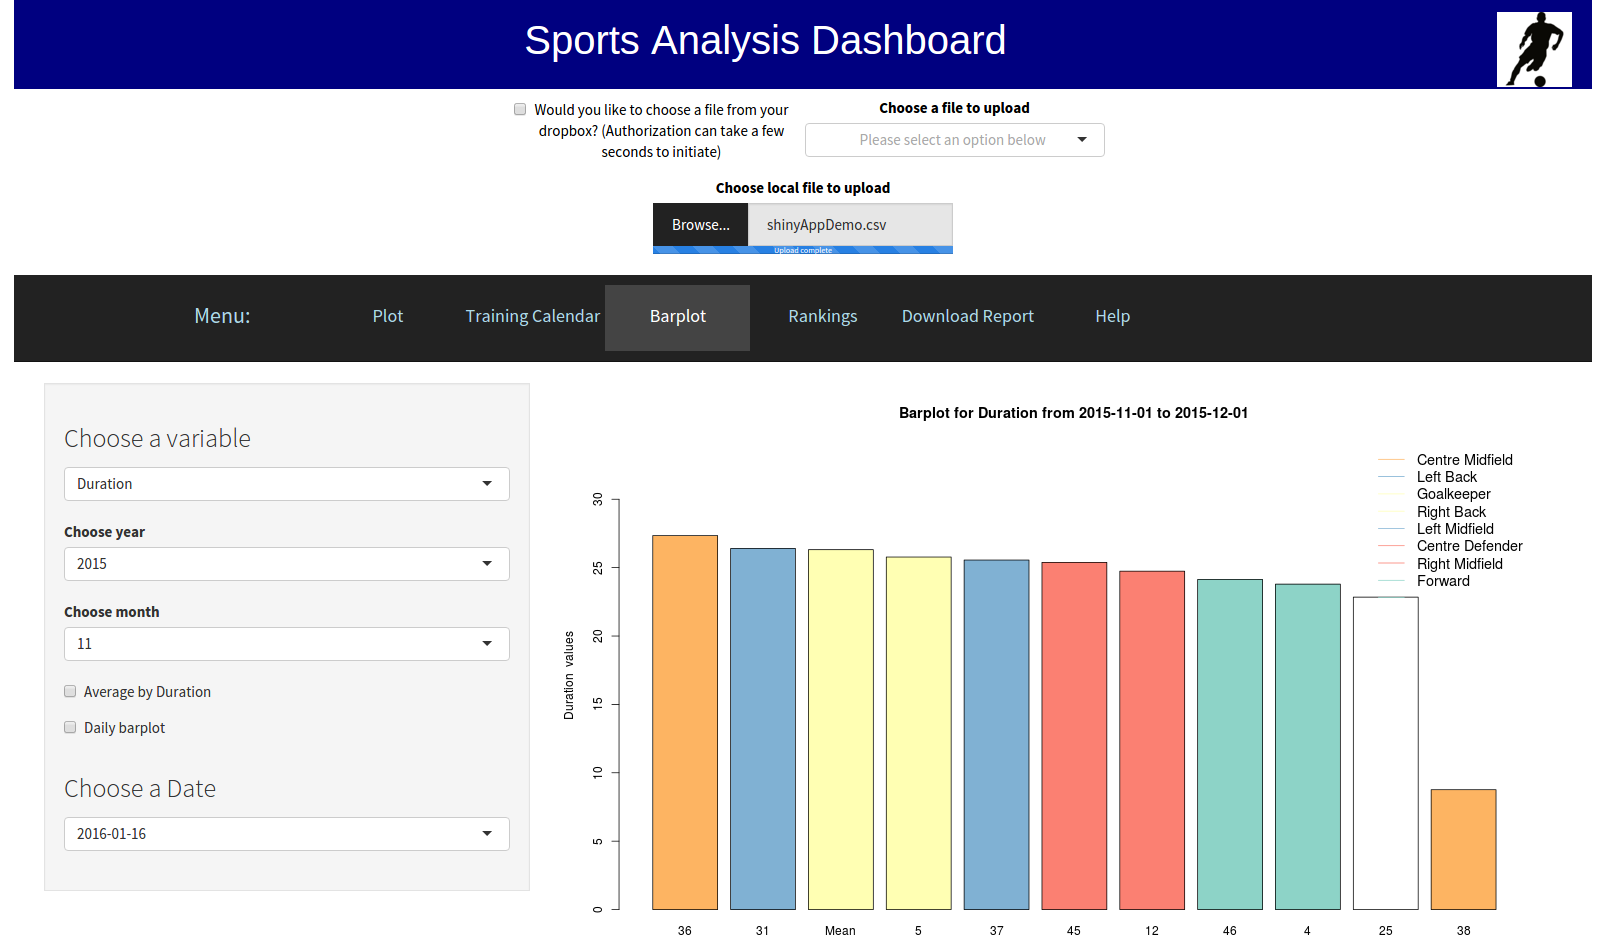
\includegraphics[width=0.8\linewidth, height=9cm]{Images/CoverPage.png}
		\end{figure}
	}
	\maketitle
	
	
	\newpage
	\vspace*{\fill}
	I hereby certify that this material, which I now submit for assessment on the programme of study leading to the award of degree is entirely my own work and had not been taken from the work of others save and to the extent that such work has been cited and acknowledged within the text of my work.
	\hfill\break	
	\newline
	Signed:\hspace{0.2cm} \makebox[1.5in]{\hrulefill}
	\hspace{0.4cm} ID no:\hspace{0.2cm} \makebox[1.5in]{\hrulefill}     
	\newline
	Date:\hspace{0.2cm} \makebox[1.5in]{\hrulefill}
	\vspace*{\fill}
	\newpage
	
	\begin{abstract}
		This project comprises of a statistical analysis and an investigation into visualization techniques of a large data set obtained from GPS tracking units. The data originated from a competitive soccer team and was not simulated, hence challenges such as missing data, high dimensionality and possible outliers were all present when attempting to perform the analysis. The main goal of the visualization of the data was to develop a general tool that could offer insights into player performance and training intensity based on a dataset that can be uploaded by a coach. The Shiny package in R was used to achieve this due to it's natural fit to the nature of the problem. The main goal of the statistical analysis of the data was to provide an insight to how a variable in the data, New.Bodyload, can be interpreted and reconstructed using other variables in the data that are more familiar to coaches and athletes.
		
	\end{abstract}
	\tableofcontents
	
	\newpage	
	\chapter{Introduction}
	\section{Motivation}
In recent years, the vast majority of major sports teams have made the choice to
set up a dedicated data analytics department in order to boost the performance
of their athletes. Statistical analyses are now motivating many decisions that in the past would have been reserved solely for instinct and experience \cite{StatsInSport}. This is due to the fact that the volume of data available to sports teams is increasing rapidly and the storage capacity for this data has become a reality in recent years \cite{GrowthOfStorageCap}.\newline

A barrier has risen for sporting teams now attempting to utilize this data: how can patterns in these vast amounts of data be extracted to give meaningful and interpretable conclusions about team performance? This is a real challenge, due to the scale of the problem. If a dataset has 70 different variables and it is desired to graphically explore the pairwise relationships of each of these variables, $\binom{70}{2}$ = 2,415 graphs need to be examined! This is clearly unfeasible and so more sophisticated techniques need to be employed in order to systematically examine and analyze the data. This is the main motivation behind this project. 

\section{Data}
I used a single dataset throughout this project that was obtained from a professional soccer team. The data was generated from GPS devices developed by GPSports, a company involved in both the development of such devices as well as providing interpretation of the device output. GPSports report that their units typically use a 15Hz positioning sampling rate, the basic signal from which is enhanced through intelligent algorithms that use a combination of GPS signal, athlete speed, direction and activity immediately prior to the sampling point \cite{tracking.pdf}. This results in a reported \textless 1\% error in the recorded distance with respect to the true distance covered \cite{tracking.pdf}. This is important since many of the derived variables in the data depend on distance. It is also important to note that it is well documented that the instrumentation is liable to errors in the variables that it records, so all GPS data will contain some degree of inherent uncertainty due to irreducible instrumentation noise/error.\newline

In the raw dataset, there were 8028 observations of 72 variables. The data was recorded over the period 22/01/2015 - 16/01/2016, with 129 unique training dates in that period. Each observation held the variables recorded during a distinct drill that an athelete had performed. The observations were recorded for 50 different athletes. The maximum number of unique training dates for any one athlete was 91, the minimum was 1 and the mean was 33.42. The variables recorded were diverse, including drill names, drill times, heart rate data, speeds the athlete achieved, metabolic information as well as zonal variables which provide the details of the activity within a certain threshold, for example the time spent running above 5m/s.







	
	\newpage
	\chapter{Statistical Analysis}
	\section{Data Preprocessing}
The preprocessing file for this project can be found on Github \cite{PreprocessingFile}. The data provided for this project was in csv format, meaning that a large portion of the preprocessing work was already completed. I chose to use R for almost all of the analysis performed in this project due to its flexibility and power in manipulating and analyzing large data sets. Once I had read in the csv file as a data frame using the read.csv function, the first step taken was to use the str() function in R to obtain an overview of the variables present in each column of the data frame. At a glance it appeared that some columns had been populated with zeros and the summary() function revealed that was the case. The columns HR.Training.Effect, Session.RPE and Sprint.Max.Acceleration were subsequently removed from the data frame. Two columns, Work.Rate.Interval.Count and Work.Rate.Interval.Duration were found to be duplicates of each other and so Work.Rate.Interval.Duration was also removed. The date column was then converted from type Numeric to type Date with the format dd/mm/yyyy.

\subsection{Outliers}
	Since New.Bodyload was the main variable of interest in this project, I began by exploring its distribution in the data set. I found one extreme outlier with a value of 14,165.74, more than 70 sample standard deviations away from the sample mean. Upon further inspection, this data point was deemed to be either a mis-calibration of the GPS unit or some other error since the maximum speed recorded was 101.02Km/h and most other columns contained anomalous information, and so this data point was removed. 11.1\% of the data was found to lie outside $ \pm $1.5*interquartile range, which is a region associated with outliers in most analyses. These were the points that had a value of New.Bodyload\textgreater150, shown in Figure 2.2. Manual inspection of these points didn't reveal any definite indication of mis-calibration of the equipment, however they looked anomalous in the data set as seen in the density plot below.
\hfill\break
\newline
I also explored the values of New.Bodyload that were relatively small in the dataset. The 0-1 bin in Figure 2.1 appears to display a break in the trend of New.Bodyload values. As noted in the data exploration section, New.Bodyload will not be zero if the unit records any acceleration with a normalized magnitude greater than 0.25g. The GPSports  site states ``Accelerations above, and decelerations below the configurable threshold are reported as events'' \cite{GPSportsVariables}. GPSports also report that accelerations from 2g-6g are reported as low impact accelerations and that ``Several thousand low intensity impacts may be seen during a football match" \cite{GPSportsVariables}. This gives a minimum of 11 low intensity impacts per minute, which suggests that at least one impact will register on average for 6 every seconds of match intensity training. This indicates that there should be very few values of New.Bodyload that are 0 and so values close to zero may be the result of a mis-calibration or other error. This explanation may account for the observed frequency in the 0-1 bin.

\begin{figure}[h]
	\centering
	\begin{minipage}{.45\textwidth}
		\centering
		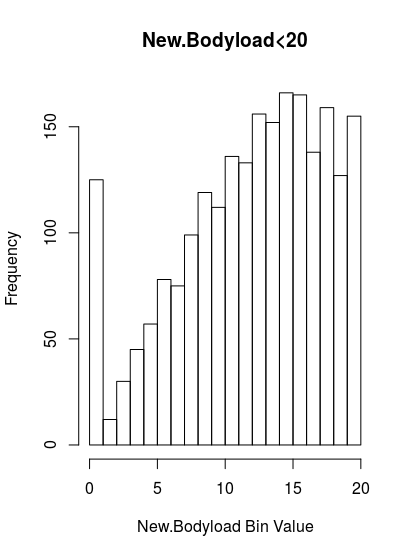
\includegraphics[width=.8\linewidth, height=6cm]{Images/NBLHistSmallVals.png}
		\captionof{figure}{New.Bodyload small values}
		\label{fig:NBLSmall}
	\end{minipage}%
	\begin{minipage}{.5\textwidth}
		\centering
		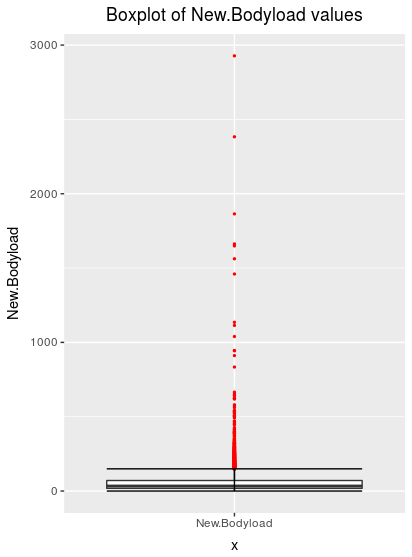
\includegraphics[width=.8\linewidth, height=6cm]{Images/NBLBoxPlot.png}
		\captionof{figure}{New.Bodyload large values}
		\label{fig:NBLLarge}
	\end{minipage}
\end{figure}
\break\hfill
\newline
The other variable that contained outliers was Duration, which is fundamental to the data along with Distance. A box plot of Duration revealed some extreme outliers with values of 641.35,609.40,603.96 and 590.90 minutes. This equates to a ten hour training session which seems impossible physically. A more likely scenario is that the units were accidentally left on after the drills had been completed. This theory is backed up by the fact that these values were all found to have occurred on the same date at the same session time. They were subsequently removed from the data set.

\begin{figure}[h]
	\centering
	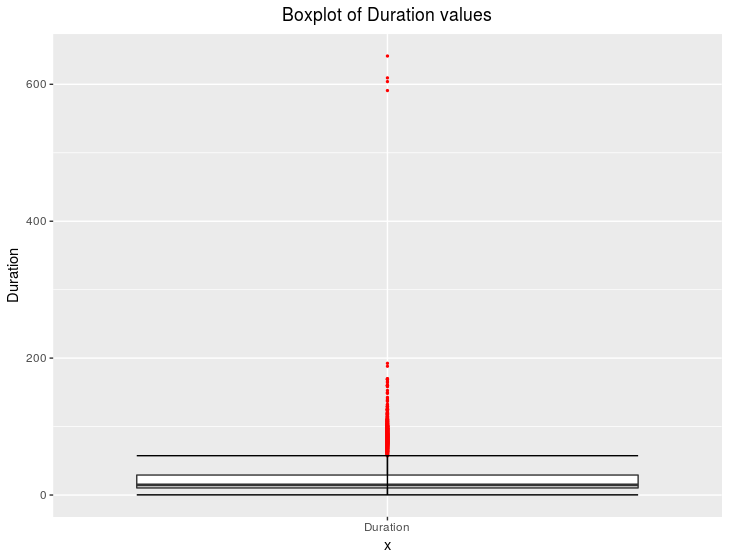
\includegraphics[width=0.6\linewidth, height=7.5cm]{Images/DurationOutliers.png}
	\caption{Extreme values of Duration variable}
\end{figure}

On the basis of these findings, I decided to carry out two analyses, one with suspected outliers and one without because I could not fully justify removing the data containing extreme values of New.Bodyload.


\section{Data Exploration}
The data exploration began with looking up GPSports' 101 page containing a summary of how the variables in the data set are constructed \cite{GPSportsVariables}. An essential part of data science is understanding how the data has originated because sometimes variable names only tell half the story. The motivation of the analysis was to offer an insight into which predictors influence the New.Bodyload variable. GPSports provide the details of how Bodyload (the old version of New.Bodyload) is derived in their FAQ \cite{NewBodyloadFAQ}. They are given as follows: 
\begin{enumerate}
	\item Initialize the BODYLOAD count to 0
	BL = 0.0
	\item Calculate the Magnitude of the Acceleration Vector for the current acceleration
	sample ie. ax, ay and az.
	\[V =\sqrt{ax^2+ay^2+az^2}\]
	
	\item Normalize the Magnitude Vector by subtracting a notional 1G
	\[NV = V – 1.0 G\]
	\item If the Normalized value is less than 0.25 G then go to step 2.
	\item Calculate the unscaled ‘BODY LOAD’ (USBL) contribution for this acceleration vector as follows:
	\[USBLC = NV + (NV)^3\]
	\item Calculate the scaled ‘BODYLOAD’ taking into account the accelerometer logging rate (100Hz) and Exercise factor (EF)
	\[SBLC = USBLC / 100 / EF\]
	Note: The Exercise Factor (EF) has been chosen so 1 hour of training activity gives a
	‘BODYLOAD’ score of roughly. This will vary depending on the individual and sport.
	\item Calculate the total ‘BODYLOAD’ as the accumulation of the scaled ‘BODYLOAD’ count
	\[BL = BL + SBLC\]
\end{enumerate}
	The idea is that New.Bodyload is an accumulative variable that essentially aggregates the extent of the force placed on the body of a player during a training session or match. This is a useful starting point for the analysis as any models constructed should ideally explain in simpler terms the motivation of this variable as the construction of the variable would not be intuitive to most people. It follows from the construction of the bodyload variable that it varies with time. This is an issue when moving to the model building phase as each measurement of New.Bodyload is taken on a different scale, namely the duration of the exercise. Treating New.Bodyload as a random variable, the consequence of this is that the observations of New.Bodyload do not come from the same distribution. One way to deal with this would be to take a time series approach to the data and interpolate values in between the non-uniformly spaced data points to give uniformly spaced values for each athlete, however in practice since the data is sparse, this would not be feasible. 
\hfill\break
\newline
Another way of looking at the New.Bodyload variable is by treating the normalized acceleration magnitude vector NV as a random variable with some positive continuous distribution. The New.Bodyload variable can then be rewritten as: \[BL=\frac{1}{100(EF)}\sum_{i=1}^{N(t)} {(NV_i+NV_i^3)} \]
where N(t) is the number of normalized acceleration vectors observed beyond the threshold stated in 4. recorded in time t. $NV_i$ is the i$_{th}$ normalized acceleration magnitude that registered beyond the threshold and $NV_i + NV_i^3$ should independent from N(t). If each of the acceleration vectors $ax,ay$ and $az$ follow a normal distribution, then $NV_i$ should follow a chi distribution with three degrees of freedom. Further discussion of the consequences of this is offered in the conclusion in section 2.4.1.
\hfill\break
\newline
The GPSports website mentions that it could be useful to divide each New.Bodyload observation by the associated duration to give a new variable offering a better comparison between athletes \cite{GPSportsVariables}. I initially considered modeling the scaled variable, with the alternative of including the duration variable in the statistical models as a predictor. Duration is obviously a key variable in determining the value of New.Bodyload for a player, however if it is included in a model then we can also infer the extent to which it motivates New.Bodyload relative to the other variables in the model, which is useful information. This information would be lost when predicting New.Bodyload/Duration so the variable was left unscaled for the analysis. If this was a question of prediction rather than inference then both models would have been explored. Density plots of New.Bodyload and New.Bodyload/Duration are shown in figure 2.3.

\begin{figure}[h]
	\centering
	\begin{minipage}{.5\textwidth}
		\centering
		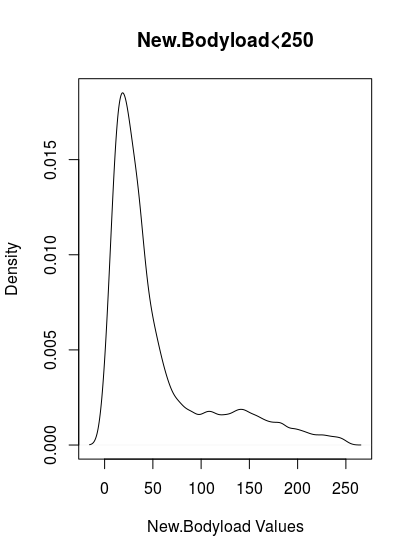
\includegraphics[width=.8\linewidth, height=7cm]{Images/NBLDensityPlot.png}
		\captionof{figure}{New.Bodyload Density Plot (94\% of data)}
		\label{fig:test1}
	\end{minipage}%
	\begin{minipage}{.5\textwidth}
		\centering
		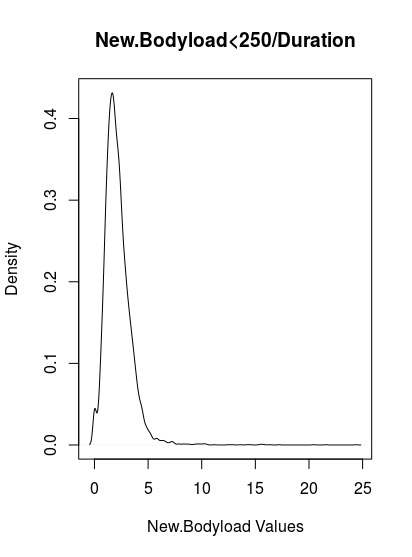
\includegraphics[width=.8\linewidth, height=7cm]{Images/NBLDivDurDensityPlot.png}
		\captionof{figure}{New.Bodyload/Duration Density Plot (94\% of data)}
		\label{fig:test2}
	\end{minipage}
\end{figure}
\hfill\break
\newline
From the information provided, it is clear that New.Bodyload should have some dependence on any acceleration related variables in the data.

\subsection{Duplicated/Missing Values}
As part of the data cleaning process, duplicated/missing values were searched for in the data. This was easily carried out using simple R functions.
\begin{lstlisting}[language=R,basicstyle=\tiny]
TRUE%in%duplicated(anonymisedData)
[1] FALSE
naPresent=lapply(names(anonymisedData),function(x)TRUE%in%is.na(anonymisedData[,x]))
which(unlist(naPresent))
integer(0)
\end{lstlisting}
There were no duplicated values in the data and no NA values in the data. The next question to ask was if there were any missing values in the non-numeric columns. 
\begin{lstlisting}[language=R,basicstyle=\tiny]
nonNumericCols=names(anonymisedData)[!names(anonymisedData)%in%numericCols]
missingVals=lapply(nonNumericCols,function(x)TRUE%in%(''%in%anonymisedData[,x]))
missingVals=nonNumericCols[which(unlist(missingVals))]
missingVals
[1] "Drill"    "Position" "Day.Code" "Squad"  
countMissingVals=lapply(missingVals,function(x) sum(''==anonymisedData[,x]))
rbind(missingVals,round(unlist(countMissingVals)/nrow(anonymisedData)*100,3))
   [,1]      [ ,2]         [,3]     [,4]    
 "Drill"  "Position"  "Day.Code"  "Squad" 
"21.926"     "0.224"     "2.305" "38.607"
\end{lstlisting}
The percentages shown could be an issue if using these variables later in the analysis. The drill variable is the most notable of these as it would make sense that high intensity drills should have higher values of New.Bodyload, so the categorical drill variable could appear in models and imputing missing values may have been worthwhile.

\subsection{Training Frequency}
Exploring the frequency at which the players trained was the next step taken. Periodic trends are often present in longitudinal data which can have consequences for the analysis. It could be the case that drills carried out in the morning tend to produce higher values of New.Bodyload relative to those carried out in the evening, for example. The density plots in Figures 2.8-2.10 show how frequently the player trained hourly, daily and monthly (normalized for time zone).\hfill\break
\begin{figure}[h]
	\centering
	\begin{minipage}{.32\textwidth}
		\centering
		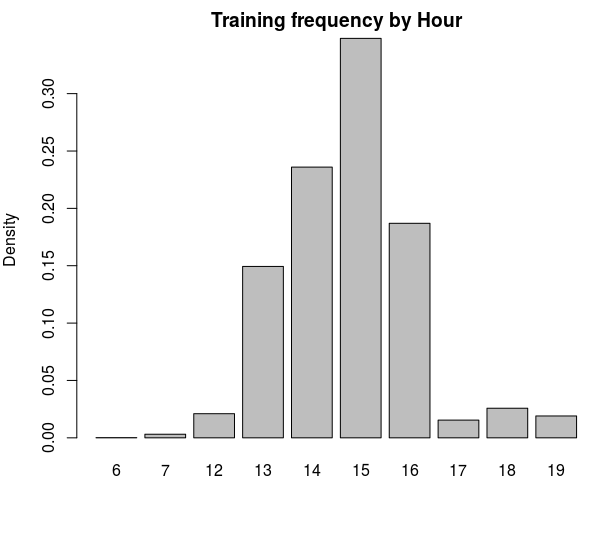
\includegraphics[width=1\linewidth, height=6.5cm]{Images/TrainingByHour.png}
		\caption{}
	\end{minipage} %
	\begin{minipage}{.32\textwidth}
		\centering
		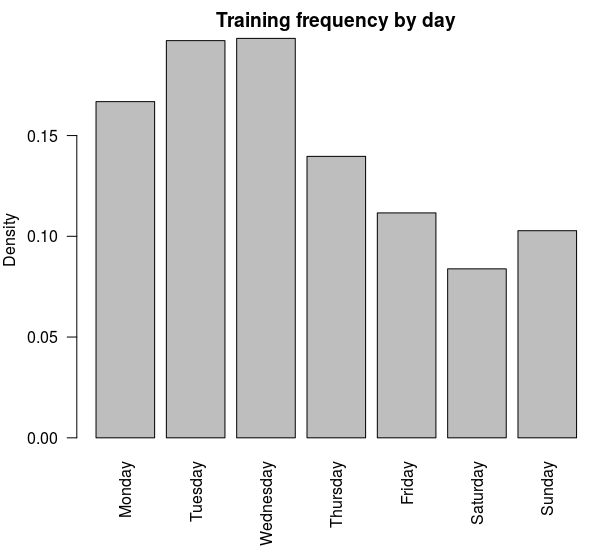
\includegraphics[width=1\linewidth, height=6.5cm]{Images/TrainingFreqDay.png}
		\caption{}
	\end{minipage} %
	\begin{minipage}{.32\textwidth}
		\centering
		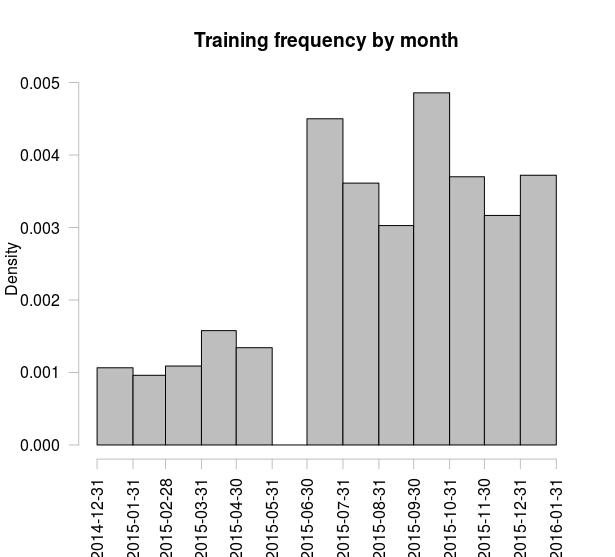
\includegraphics[width=1\linewidth, height=6.5cm]{Images/MonthlyDrills.png}
		\caption{}
	\end{minipage}
\end{figure}
\break\hfill
\newline
The plots reveal some interesting information: it seems like players are likely to train from 1pm-4pm, so it could be the case that if multiple trainings are carried out per day, New.Bodyload values will be lower in the 17:00 - 19:00 bracket. There is also a clear trend of training more often earlier in the week, which provides a sanity check as matches are usually held on Saturdays when the training frequency is lowest. The last plot arguably reveals the most information, as it appears that players train at a much higher frequency in the later months of 2015. The absence of data in June represents the players' break between the end of the 14-15 season to the beginning of pre-season training for 15-16. Figure 2.8 was worth investigating further, so I generated a plot of mean duration per month.\hfill\break
\newline
\begin{figure}[h]
	\centering
	\begin{minipage}{.48\textwidth}
		\centering
		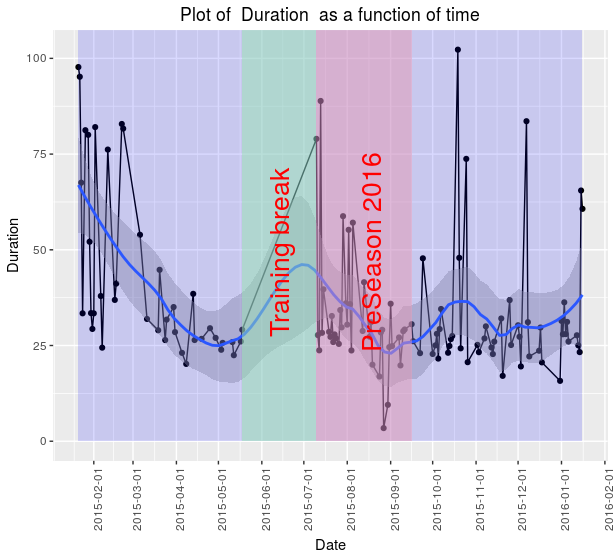
\includegraphics[width=1\linewidth, height=7cm]{Images/DurationForSeason.png}
		\caption{Mean Duration value per Date}
	\end{minipage} %
	\begin{minipage}{.48\textwidth}
		\centering
		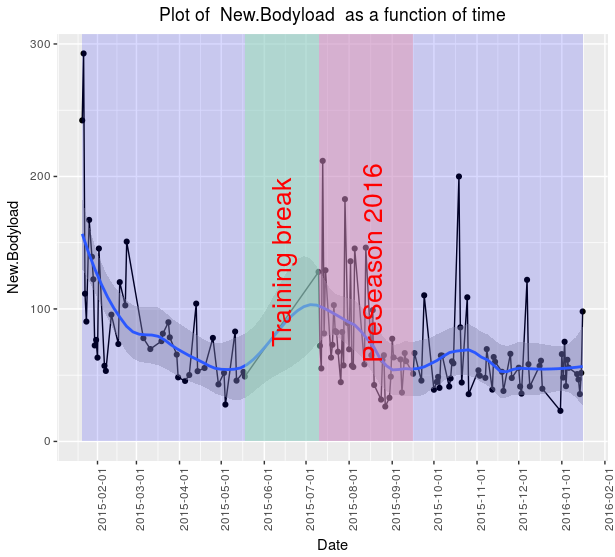
\includegraphics[width=1\linewidth, height=7cm]{Images/NBLTime.png}
		\caption{Mean New.Bodyload value per Date}
	\end{minipage} 
\end{figure}
Figure 2.11 reveals that the mean duration of training sessions was longer in the early months of 2015 but the sessions were less frequent. Figure 2.12 shows that the mean New.Bodyload value on any given date is higher for high duration exercises, however this information can be misleading as New.Bodyload is accumulative and so the mean value does not allow for comparisons (5 observations of New.Bodyload values of 10, each over a duration of 10 minutes gives a mean value of 10, whereas 1 observation of a New.Bodyload value of 50 over a duration of 50 minutes gives a mean value of 50, despite the same accumulative value of New.Bodyload). To really understand how New.Bodyload is varying over time, a plot of the accumulative value of New.Bodyload/Duration per date is required, displayed in Figure 2.11. 

\begin{figure}[h]
	\centering
	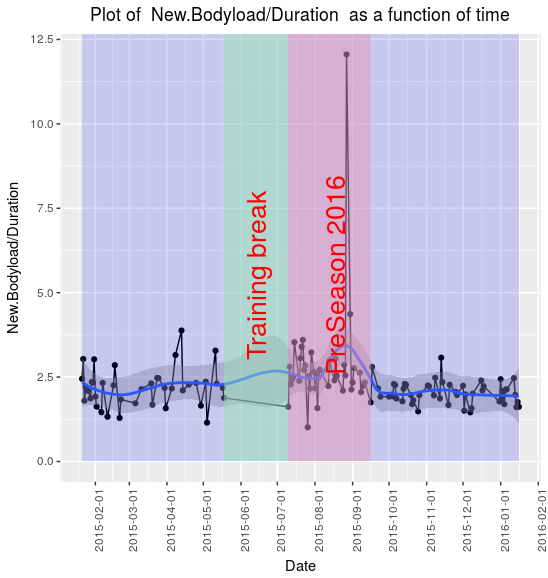
\includegraphics[width=0.6\linewidth, height=8cm]{Images/NBLScaledByDuration.png}
	\caption{New.BodyLoad scaled by Duration}
\end{figure}

Figure 2.11 yields a lot of information: when New.Bodyload is scaled by duration, its mean value per date appears constant $\pm$ some noise term. This indicates that New.Bodyload does not significantly vary seasonally in relation to the duration of drills. It is clear from this exploration that New.Bodyload has a significant dependence on the Duration variable (high duration implies high New.Bodyload), but it may not have a dependence on the date at which it was recorded. This agrees with the GPSports documentation on the variable.

\subsection{Correlations and Predictors}
The next part of the data exploration focused on examining possible predictors of New.Bodyload. I first decided to explore non-numeric predictors. Position was first to be explored: it could be the case that certain positions have a natural tendency to produce higher values of New.Bodyload.
\begin{figure}[h]
	\centering
	\begin{minipage}{.48\textwidth}
		\centering
		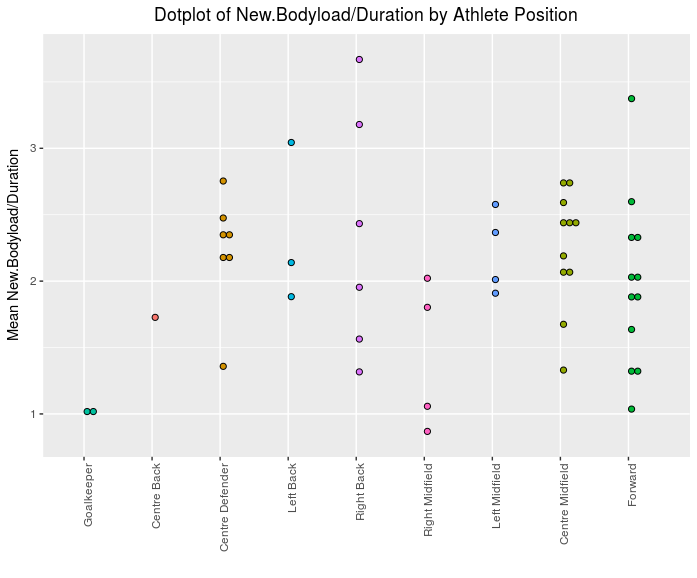
\includegraphics[width=1\linewidth, height=6.5cm]{Images/NBLPosDotPlot.png}
		\caption{Mean NBL/Duration values of each athlete grouped by Position}
	\end{minipage} %
	\begin{minipage}{.48\textwidth}
		\centering
		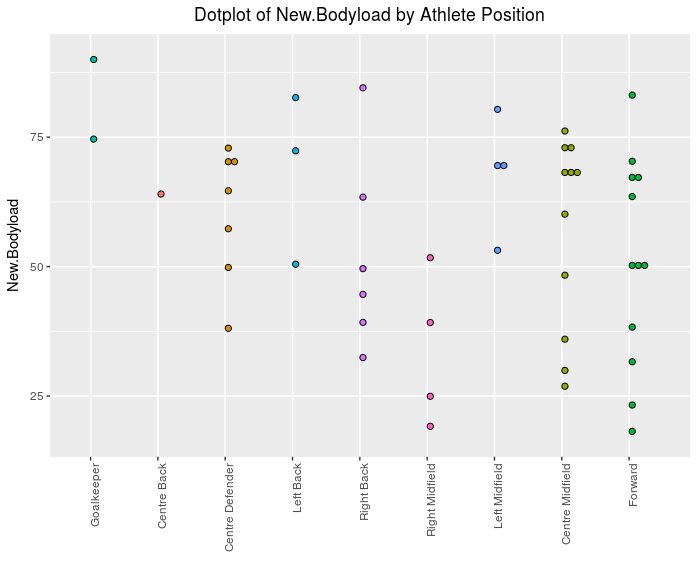
\includegraphics[width=1\linewidth, height=6.5cm]{Images/UnscaledDotplot.png}
		\caption{Mean NBL values of each athlete grouped by Position}
	\end{minipage} 
\end{figure}
Again here it made sense to first scale New.Bodyload by duration in order to be able to compare the values (Figure 2.13). The graphs reveal that New.Bodyload varies highly within each position and there is no clear trend of certain positions exhibiting significantly different values of New.Bodyload relative to others. Since football teams will typically train as one big group, it makes sense that players will experience similar values of New.Bodyload and the implication is that this variable will not be a good predictor of New.Bodyload.
\hfill\break
\newline
Drill was the other non-numeric variable examined. As discussed in 2.2.1, 22\% of values were not provided. A quick summary of the variable revealed too much ambiguity in the drill names for them to be effective predictors, for example ``3 Colour Possession" and "3 Colours Possession 1/4 Pitch 7v7v7" might be distinct from each other but it is not clear if this is the case. This would lead to confusion when attempting to make inferences about the variable.\hfill\break
\newline
The other predictors provided in the data that were worth exploring were all numeric. I began by building a correlation matrix (Figure 2.14). This gave an indication of pairwise linear associations between variables. The matrix illustrates that there are strong linear associations between many of the variables. Based on this plot I discovered that some variables in the data could be almost fully explained by linear combinations of other variables, which lead to the removal of Equivalent.Distance, Max.HR, Sprint.Count, Work.Rate.Interval.Count and Metabolic.Load..absolute. from the data for the modeling phase, the reason being that when constructing general linear models using ordinary least squares, multicollinearity of predictors leads to the ordinary least squares estimator ${\displaystyle {\hat {\beta }}_{OLS}=(X^{\mathsf {T}}X)^{-1}X^{\mathsf {T}}y}$, which does not exist because ${\displaystyle X^{\mathsf {T}}X}$ either cannot be inverted or is inverted in such a way that numerically unstable estimates of the regression coefficients result (small changes in X can result in large changes to the estimated regression coefficients). It appeared that New.Bodyload had a linear relationship with a large number of variables in the model which meant that a linear model should be able to explain how the variable is constructed reasonably well. It also suggested that there was strong multicollinearity between many of the possible predictors, which needed to be further addressed at the modeling stage.
\begin{figure}[h]
	\centering
	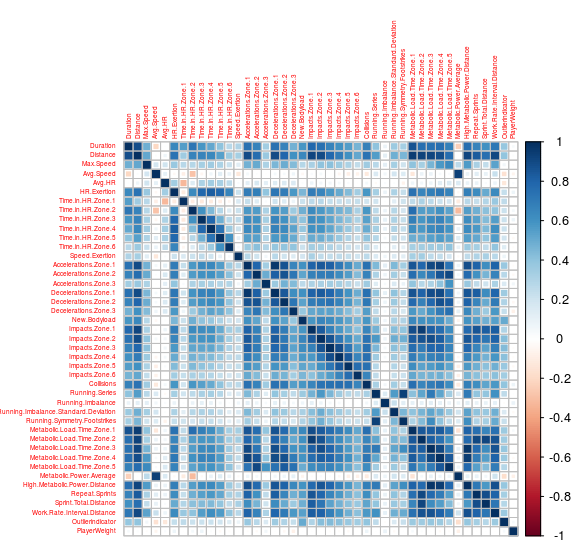
\includegraphics[width=0.8\linewidth, height=10cm]{Images/CorrelationPlot.png}
	\captionof{figure}{Correlation Matrix of Numeric Variables}
\end{figure}
\hfill\break

\section{Data Modeling}
For the sake of simplicity of building statistical models I made the assumption that the observations were independent of each other. As discussed in section 2.1.1, I chose to build two sets of models, one using the data with suspected outliers and the other using the data with suspected outliers removed. I also partitioned my data into train and test sets of size 80\% and 20\% of the full data set respectively. The reason for this was to ensure that I could check that the models that I built were not over fitting the data and giving false indications of their usefulness in making inferences about the data. Assuming that New.Bodyload $(Y)$ is some function of the predictors $(X)$, $Y=f(X)+\epsilon$, (where $\epsilon$ is assumed to be a random error term, which is independent of X and has mean zero), the aim of the data modeling is to find a function $\hat{f}(X)$ which approximates the true function    $f(X)+\epsilon=Y \approx $ $\hat{Y} = \hat{f}(X)$. Ideally this model will be able to answer the following questions, (recommended in the Tibshirani \& Hastie book ISLR as key questions for any inference problem)\cite{ISLR}: 
\begin{enumerate}
\item Which predictors are associated with the New.Bodyload, the response variable?
\item What is the relationship between New.Bodyload and each predictor (if any)?
\item Can the relationship between New.Bodyload and each predictor be adequately summarized
using a linear equation, or is a more complex relationship more informative?
\end{enumerate}
\subsection{Intended Outcomes}
During the modeling stage of the data, I aimed to achieve a number of outcomes: 
\begin{enumerate}
	\item \emph{Explore Dimension Reduction Techniques}. There were $\approx$60 variables in the data frame available for use in the modeling phase, which could lead to a model that is highly predictive of New.Bodyload but difficult to interpret. Dimension reduction of the data has the effect of limiting the number of variables used in statistical models which can help account for most of the variance of New.Bodyload while also explaining how New.Bodyload is constructed in a concise manner.
	\item \emph{Based on 1., an interpretable model was desired.} This ruled out highly flexible models such as random forests. The models I explored included 
	linear models and tree based models.
	\item Once the models had been constructed, I needed a method of evaluating and comparing them. Adjusted $R^2$ values for linear models and Mean Squared Error usually gave a good indication but I also explored other methods of comparing models.
	\item Explore the usage of basis functions to develop separate models for fundamentally different groups in the data.
\end{enumerate}
The construction and analysis of the models discussed in the next section relate to the data with suspected outliers removed, with a section at the end discussing how the modeling process with outliers affected the analysis. Once the suspected outliers were removed $\approx$93\% of the data available for this project remained.

\subsection{Linear Models}
 Linear models are useful for both prediction and inference due to their simple form, theoretical support, quick computation time, flexibility in incorporating interaction terms and transformations of predictors, ability to include dummy variables for categorical variables and straightforward interpretation \cite{ESL}. Linear models are based on four main assumptions: 
\begin{enumerate}
\item Linearity of ${f}(x)$. Linear models are parametric, where the functional form of $f$ is assumed to be $f(X)=Y=\beta_0+\beta_1X_1+...+\beta_nX_n$, where each $X_i$ is the value of the $i_{th}$ predictor and each $\beta_i$ is a scalar value which can be thought of as the weight of the corresponding predictor in estimating New.Bodyload.
\item Constant variance of residuals (homoscedasticity). Homoscedasticity implies that different response variable observations have the same variance in their corresponding residuals, regardless of the values of the predictor variables. If the residuals of the predictions did not have constant variance, then the standard error of the residuals will be biased. Since the standard error is important when conducting significance tests and calculating confidence intervals of coefficient values, biased standard errors result in misleading conclusions regarding New.Bodyload. Since linear models minimize MSE over all observations, it makes sense that the residuals produced by linear models should not be biased over some regions but not others.

\item Independence of residuals. This is especially relevant in this analysis as time series data can have seasonal effects which lead to correlated residuals. If the residuals are not independent of each other, this can mean that the linear assumption is incorrect.

\item Normality of residuals. This assumption is made so that the residuals are unbiased and are no more likely to overestimate the response variable as underestimate.
\end{enumerate}

\subsubsection{Simple Linear Regression}
One of the first approaches I took to modeling the data was to fit a simple linear model. The results of fitting the linear model are shown in Figure 2.15. 
\begin{figure}
	\centering
	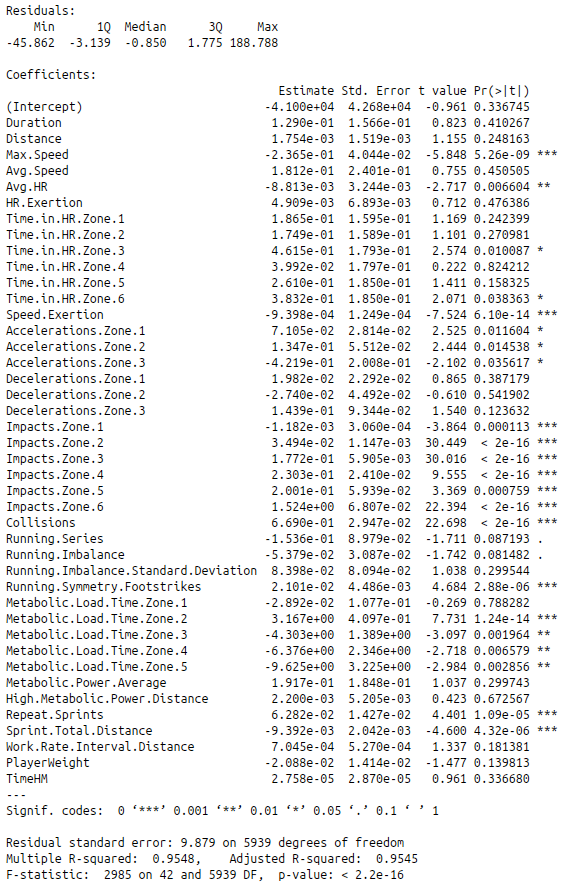
\includegraphics[width=.9\linewidth]{Images/SimpleRegressionOutput.png}
	\captionof{figure}{Linear Model Summary}
\end{figure}
The figure given for Multiple R-squared represents the ratio of the explained variation of New.Bodyload to the total variation of New.Bodyload, according to the following formula:
\[
Multiple \,  R^2=\frac{\sum_{i=1}^{n}(\hat{y_i}-\bar{y})^2}{\sum_{1}^{n}(y_i-\bar{y})^2} 
\]
and the value of adjusted R-squared gives a more accurate estimate of how well the data is fitting the model by taking into account the number of predictors used:
\[
Adjusted \, R^2=1-[\frac{(1-R^2)(n-1)}{n-k-1}]
\]

The high value of $R^2$ here indicates that the model is fitting the data well, however the residual plot associated with this model shows that the model predicts more accurately on small values of New.Bodyload compared to large values of New.Bodyload. A normal quantile plot also indicates that the errors associated with the predictions of New.Bodyload are not normal, which means that the standard errors associated with the predictors in the model may be inaccurate, since the calculations of standard errors and significance tests for coefficients are all based on the assumptions of homoscedasticity, independence and normality of residuals. The runDiagnostics function, found on Github \cite{ModellingWithoutOutliers}, was used to generate the plots shown in the figures 2.16-2.18.
\hfill\break
\begin{figure}[h]
	\centering
	\begin{minipage}{.33\textwidth}
		\centering
		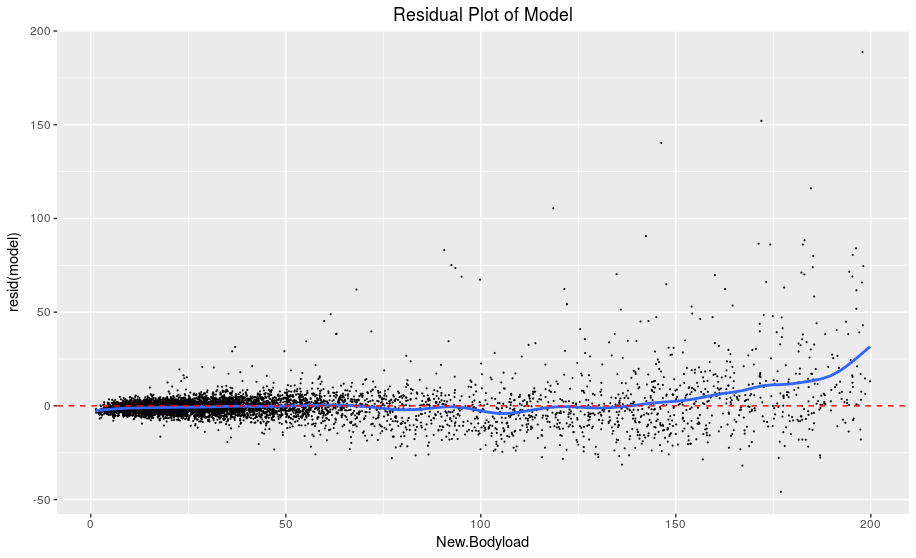
\includegraphics[width=.9\linewidth, height=5cm]{Images/SimpleLinearResidual.png}
		\captionof{figure}{Linear Model Residuals}
	\end{minipage}%
	\centering
	\begin{minipage}{.33\textwidth}
		\centering
		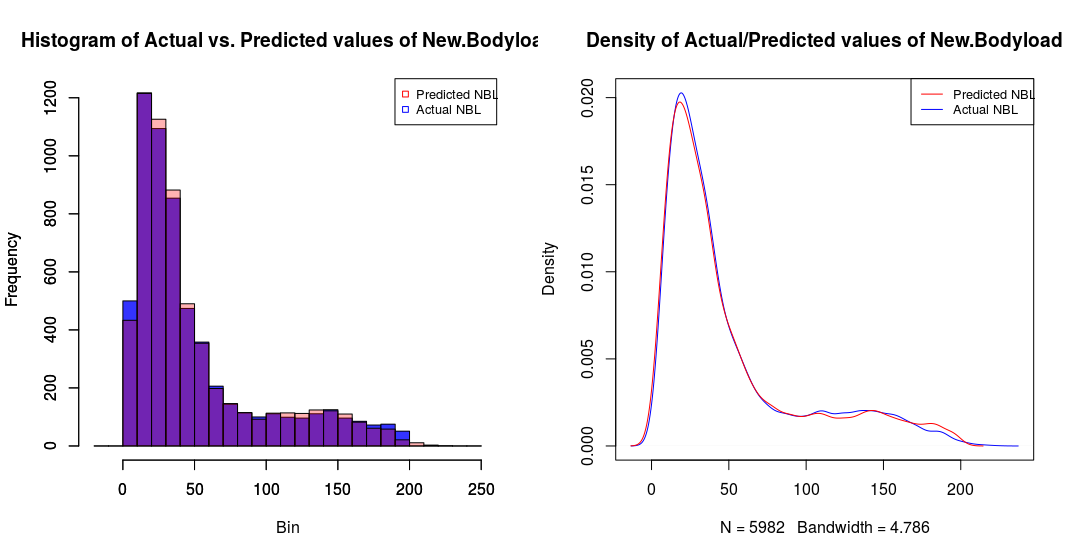
\includegraphics[width=.9\linewidth, height=5cm]{Images/SimpleLinearHist.png}
		\captionof{figure}{Linear Model Prediction Densities}
	\end{minipage}%
	\begin{minipage}{.33\textwidth}
		\centering
		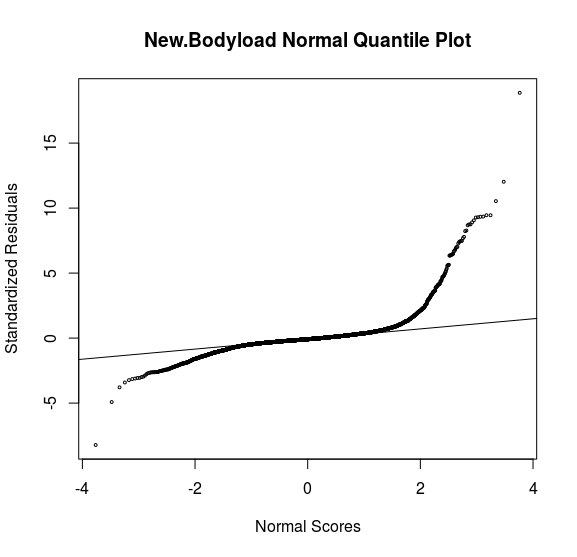
\includegraphics[width=.9\linewidth, height=5cm]{Images/QuantilePlot.png}
		\captionof{figure}{Normal Q-Q Plot}
	\end{minipage}
\end{figure}

Since the goal of this analysis is inference, this model is not useful because it contains too many predictors and its coefficients cannot be accurately estimated. The model summary shows that variables like Distance and Duration have a small t-statistic in the model which strongly goes against intuition. Clearly, there is a lot of room for improvement for this model, but it use lies in its adjusted $R^2$ and MSE values, which set a benchmark for other models. Since adding predictors to a model can only increase these values, a challenge is now presented in approaching this value using as few predictors as possible.
\hfill\break
\newline
As discussed in section 2.2.3, the effects of multicollinearity should be explored in this problem. Each predictor weight in the model, $\beta_i$ has an associated standard error, which provides a confidence interval of the coefficient value according to the equation: $Var(\hat{\beta})=(X^TX)^{-1}\sigma^2$, given the assumption that $y_i$, the observations of New.Bodyload, are uncorrelated and have constant variance $\sigma^2$, and that the $x_i$ are fixed (non random)\cite{ESL}. As discussed in section 2.2.3, $(X^TX)^{-1}$ will have an unstable solution if columns of the matrix are almost linearly dependent and so the estimates of the standard errors of the predictors will be correspondingly unstable, hence it is desirable to have a quantitative sense of the amount of multicollinearity in a model. One way of measuring the effects of multicollinearity in predictive models is to calculate the variance inflation factor associated with each predictor in the model. The variance inflation factor can be thought of a measure of how much the variance of the estimated regression coefficient $\beta_k$ is ``inflated" by the existence of correlations among the predictor variables in the model. It can be calculated as follows: \[VIF(\beta_k)=\frac{Var(\beta_k)}{Var(\beta_k)_{min}}=
\frac{(\frac{\sigma^2}{\sum_{i=1}^{n}(x_i^k-\bar{x}^k)^2})(\frac{1}{1-(R^2)^k})}
{(\frac{\sigma^2}{\sum_{i=1}^{n}(x_i^k-\bar{x}^k)^2})}=\frac{1}{1-(R^2)^k}\]
where $x_i^k$ is the i$^{th}$ observation of the k$^{th}$ predictor and ${1-(R^2)^k}$ is the R$^2$-value obtained by regressing the k$^{th}$ predictor on the remaining predictors. This implies that strong linear dependence among the predictor x$^k$ and the other predictors results in a large $(R^2)^k$ value. This further implies that large values of $(R^2)^k$ induce a large variance in $\beta^k$, which we would rather detect and avoid \cite{VIF}. Note that if $(R^2)^k$=0, the variance will not be inflated at all (VIF=1), so orthogonal columns of the matrix $(X^TX)$ are desirable for this problem. In the simple linear regression carried out above, the vif function in the CAR package revealed that 25 out of 43 of the variables had a variance inflation factor above 10, which as a rule of thumb is considered to indicate significant multicollinearity\cite{Multicollinearity}.


\subsubsection{Forward Stepwise Selection}
The previous model indicated that many of the variables in the data were not predictive of New.Bodyload and their inclusion in the linear model had a detrimental effect on the confidence interval estimates of the model coefficients. Since the objective is inference, the ideal model is one that uses few variables but can succinctly explain a large amount of the variance associated with New.Bodyload. The Forward Stepwise Selection algorithm can be used to construct such a model. The idea is to limit linear regression to a maximum of p predictors, where each iteration of the algorithm introduces an additional predictor to the model in a greedy manner. The algorithm runs according to the following set of steps \cite{ISLR}: 
\begin{enumerate}
	\item Initialize $Model_0$ as the null model, which contains no predictors.
	\item For k = 0,...,p-1:
	\item Fit p-k models, each of which adds one new predictor to the predictors already present in $Model_k$
	\item Whichever model results in the largest reduction in RSS is set as $Model_{k+1}$
	\item Select a single best model from all of the models built.
\end{enumerate}
The algorithm is heuristic, where the optimal solution isn't guaranteed but the runtime of the algorithm is limited. I used this technique to produce 10 models, each consecutive one having one more variable than the last. The results of the models showed some variables to be significant in the restricted model which were not significant in the Simple Linear Regression, most notably Duration. It is not clear how step 5 is achieved, since in different problems ``best" can mean different things. Here I wanted a model that was highly interpretable, so among the n models, I sought a model that could explain most of the variance associated with New.Bodyload with the fewest predictors. Figure 2.19 displays the $R^2$ value associated with each model containing increasing numbers of variables.

\begin{figure}[h]
	\centering
	\begin{minipage}{.45\textwidth}
		\centering
		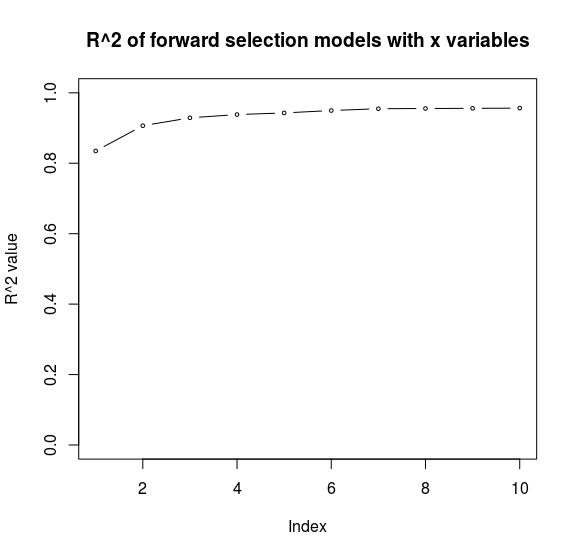
\includegraphics[width=.9\linewidth, height=5cm]{Images/ForwardSelectionPlot.png}
		\captionof{figure}{Number of predictors in model vs. $R^2$ value associated with model}
	\end{minipage}%
	\hfill
	\begin{minipage}{.45\textwidth}
		\centering
		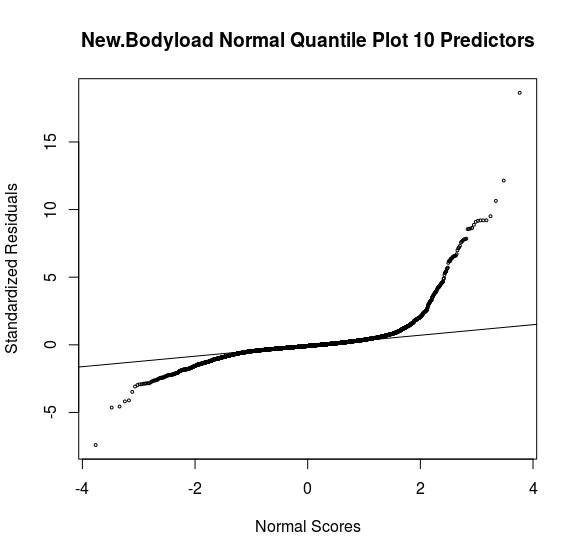
\includegraphics[width=.9\linewidth, height=5cm]{Images/QuantilePlot10Predictors.png}
		\captionof{figure}{Normal Quantile Plot for model limited to 10 predictors}
	\end{minipage}
\end{figure}
\break
Using more than ten predictors had negligible effect on increasing $R^2$ values. Figure 2.20 again revealed non-normal errors, which means once again that the coefficient estimates may not be accurate in the model. The top ten variables selected by the model were added in the following order: Impacts.Zone.2, Impacts.Zone.4, Duration, Impacts.Zone.6, Impacts.Zone.3, Metabolic.Load.Time.Zone.2, Collisions, Max.Speed, Speed.Exertion, Avg.Speed. Intuitively these variables all make sense in the model. The variance inflation factors for models containing 2-7 variables are shown in figure 2.21. Again residual diagnostics revealed heteroscedasticity was present for these models. 
\begin{figure}[h]
	\centering
	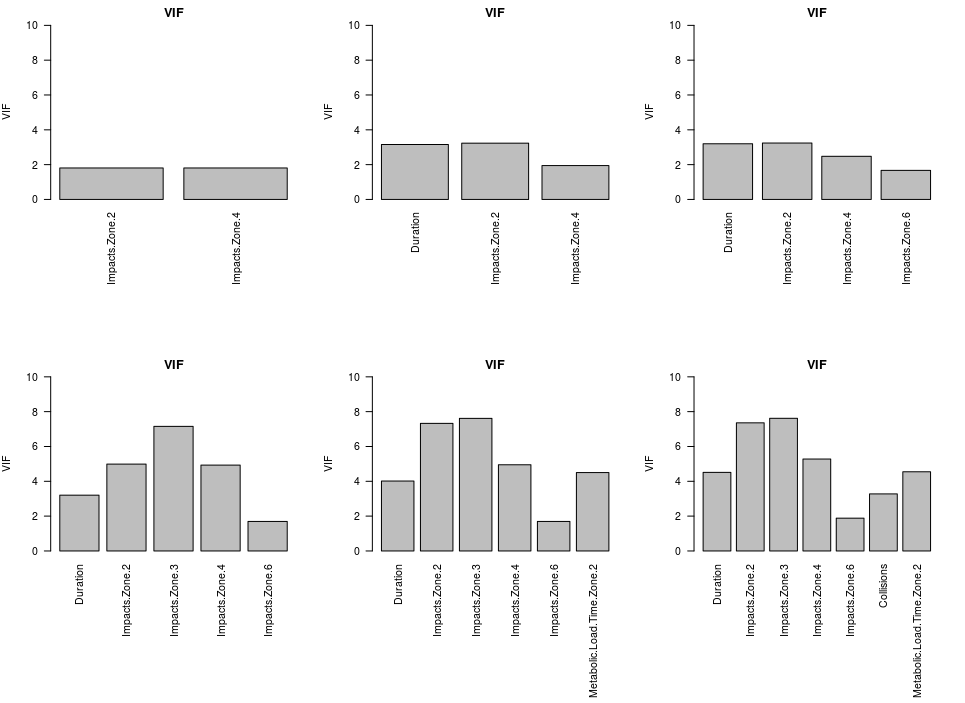
\includegraphics[width=.9\linewidth]{Images/VIFForwardSelection.png}
	\captionof{figure}{Variance Inflation factors for each Forward Selection model}
\end{figure}

\subsubsection{Best Subset Selection}
The Best Subset Selection algorithm is similar to the Forward Selection algorithm in that it chooses a subset of variables to include in a linear model. The key difference is that Best Subset Selection chooses the best linear model limited to n predictors out of \emph{all} possible ${p}\choose{n}$ models limited to n predictors (again the definition of ``best" varies with context). Given that there are 43 possible predictors in the model, this task becomes unfeasibly large for values of n greater than ~7 (32,224,114 models to compare). Forward Subset Selection revealed that a relatively large $R^2$ value can be achieved using few predictors so this technique was worth exploring. The advantage of using Best Subset Selection with this data set was that the effects of multicollinearity were automatically mitigated by the algorithm since irrelevant/noisy variables are omitted from the best model. The details of the model limited to 7 predictors using the best subset selection algorithm are shown in figure 2.22: 
\begin{figure}[h]
	\centering
	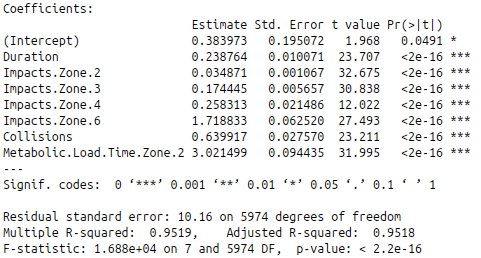
\includegraphics[width=.75\linewidth]{Images/BestSubsetSelectionConclusion.png}
	\captionof{figure}{Best Subset Selection 5 variables}
\end{figure}
\break\hfill
Diagnostic plots once again revealed that while the model captured the overall trend, there was heteroscedasticity and non-normal residuals present. 

\subsubsection {Lasso}
Another linear model explored was the Lasso. This model is an extension of Simple Linear Regression, where the coefficients are fit by minimizing the quantity \[\sum_{i=1}^{n} (y_i-\beta_0-\sum_{j=1}^{p}\beta_jx_{ij})^2 + \lambda\sum_{j=1}^{p}|\beta_j| = RSS + \lambda\sum_{j=1}^{p}|\beta_j| \]
where high values of $\lambda$  tend to penalize coefficients with relatively high values. The idea is that a well chosen lambda value shrinks some of the coefficient values to zero while leaving the coefficients that are more efficient at reducing the RSS as non-zero valued. Further details of the lasso can be found in Tibshirani and Hastie's book ISLR \cite{ISLR}. As the value of lambda was varied, variables were introduced by the lasso in the following order: Distance \& Impacts.Zone.2 (Simultaneously), Impacts.Zone.3, Collisions, Duration, Impacts.Zone.4, Metabolic.Load.Time.Zone.2, Impacts.Zone.6, Impacts.Zone.5, Metabolic.Load.Time.Zone.1.


\subsubsection{Polynomial Regression}
Polynomial regression was implemented to explore the possibility that there were strong non-linear relationships between some of the predictors and New.Bodyload. First, it was necessary to create a new data set containing non-linear transformations of each of the variables. R is suited to performing such transformations and the functions found in \cite{ModellingWithOutliers}  were used to create an additional 301 variables. For each predictor column vector X$_j$ (excluding New.Bodyload), 7 new columns were created corresponding to $X_j^i, i \in \{-4,-3,-2,-1,2,3,4\}$. First I carried out the forward selection algorithm to limit the runtime because the search space now contained 336 predictors rather than 43. Variables were included in the following order: Impacts.Zone.2, Impacts.Zone.4, Duration, Impacts.Zone.6, Impacts.Zone.3, Metabolic.Load.Time.Zone.2, Collisions,  Duration$^4$, Speed.Exertion, Max.Speed$^{-1}$. A best subset selection limited to a maximum of 5 variables yielded the model in figure 2.23.
\begin{figure}[h]
	\centering
	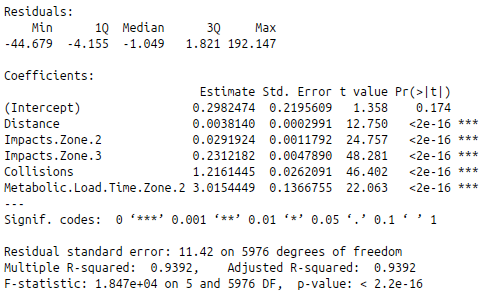
\includegraphics[width=.6\linewidth, height=6cm]{Images/PolynomialBestSubset.png}
	\captionof{figure}{Best Subset Selection With Polynomial Terms}
\end{figure}
\hfill\break
\newline
Note that only non-transformed variable appear in this model. This was not surprising as scatter plots of New.Bodyload did not indicate non-linear relationships with any of the variables flagged as strong predictors by previous models. The anova function in R, with null hypothesis stating that the two models
fit the data equally well, and the alternative hypothesis stating that the model containing polynomial terms is superior showed that each forward selection model using x variables with polynomial predictors is not significantly superior to the forward selection model with a corresponding number of linear predictors. It could have been the case that a different type of non-linear transformation could have yielded better results, however when constructing a model with the purpose of inference, using raw variables has the advantage of being highly interpretable. The project could have been extended by further exploring non-linear transformations of both the predictors and the dependent variable.

\subsubsection{Linear Regression With Interaction Terms}
Since some of the predictors in the data set were accumulative with time, their inherent reliance on Duration implied that there could be some interaction effects in the data that could be taken advantage of. Linear models discussed in previous sections all had a coefficient $\beta_j$ associated with the $j_{th}$ predictor, which represented the change in New.Bodyload corresponding to a unit increase in the predictor value, keeping all other predictors fixed. In some regression problems, it has been observed that there are synergistic effects between predictors in the model. It could be the case, for example, that increasing values of Duration could in turn increase the effect of Impacts on an athlete, so that values of New.Bodyload increase at non-constant rate per unit change in Collisions. In order to explore this, the variables that appeared in the best subset selection limited to ten variables were multiplied together to generate 66 new columns. Then best subset selection was ran with a maximum of 5 variables which yielded the model in figure 2.24.
\begin{figure}[h]
	\centering
	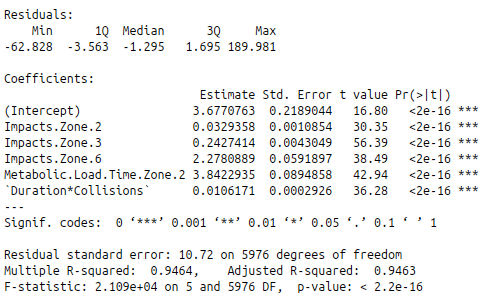
\includegraphics[width=.6\linewidth, height=6cm]{Images/InteractionModelBestSubset.png}
	\captionof{figure}{Best Subset Selection With Interaction Terms}
\end{figure}
\break\hfill
The interaction term Duration*Collisions can be interpreted as follows: for every minute that the drill lasted, each additional collision experienced in the drill over the duration of that minute increased the value of New.Bodyload by 0.0106171 ($\pm 0.0002926$).

\subsubsection{Principal Components Analysis (PCA)}
Principal components analysis is a technique which is used to reduce the dimensionality of data. The motivation behind principal components analysis is that many variables in a large data set containing correlated variables are essentially redundant. Therefore it makes sense to try and find directions in the feature space of the data in which to project the data so that the dimensions projected to contain as much variance as possible. PCA transforms the original set of (possibly correlated) predictors to a new set of linearly uncorrelated predictors. The first k principal components span the k-dimensional hyperplane that is closest to the n observations. The first principal component is a vector, $z_1$, constructed using values $\phi_{i1}$ (referred to as a loading vector) and the predictor columns such that the linear combination of the predictors of the form 
\[z_{1}=\phi_{11}X_{1}+\phi_{21}X_{2}+...+\phi_{p1}X_{p}\]
has the largest possible sample variance, subject to $\sum_{j=1}^{p} \phi_{j1}^2=1$, where $X_{i}$ represents the vector of observations of the $i_{th}$ predictor and $\phi_{i1}$ represents the i$_{th}$ entry of the first principal component weight vector. Subsequent principal components are defined in a similar fashion, with the constraint that they must be orthogonal to the previous principal components.

\begin{wrapfigure}{r}{5cm}
	\vspace{-1em}
	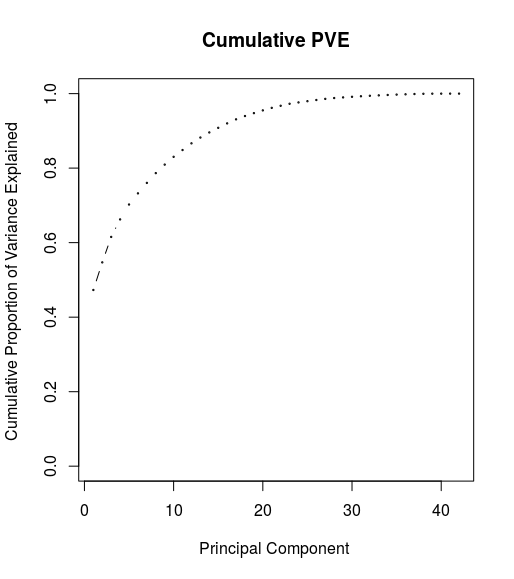
\includegraphics[height=6cm]{Images/CumulativePVEPCA.png}
	\caption{Cumulative graph of the proportion of variance explained by each principal component}
\end{wrapfigure}
Since the data used in this project contained correlations between multiple predictors, PCA was implemented in an attempt to resolve multicollinearity issues that were evident in linear models. I used the prcomp function in R to generate the principal components for this data set. Figure 2.25 shows that the first principal component was able to explain 47\% of the variance in the data, with each subsequent principal component explaining a further \textless 7\% of the variance present. Clearly the first principal component encodes a lot of information about the data relative to the remaining components. Since principal components analysis creates a new set of variables that are linearly uncorrelated, using these variables as predictors in a model could help solve the problems associated with multicollinearity experienced with other models. Keeping in mind that inference was the goal of the project, this technique was not explored in depth because principal components can be difficult to interpret. Both principal components regression and partial least squares regression were implemented on the data set to explore whether they could offer a set of uncorrelated variables that are highly predictive of New.Bodyload in a linear model. This solved the issues surrounding multicollinearity associated with the other linear models but also resulted in a set of variables that were difficult to interpret.

\subsection{Non-Linear Models}
\subsubsection{Regression Tree}
I began the data modeling by building a simple regression tree, as tree-based methods tend to be straightforward to construct and easy to interpret. Decision trees are constructed by stratifying the feature space into distinct regions which have piecewise constant predicted values of  New.Bodyload. The tree algorithm performs recursive binary splitting by selecting the predictor $X_j$ and the cut point s such that splitting the predictor space into the regions $\{X|X_j < s\}$ and $\{X|X_j \geq s \}$ maximizes the resulting reduction in RSS due to the split. This algorithm is greedy and is not guaranteed to find the best solution but it limits the search space in such a way that a solution can easily be found. Figure 2.26 shows the structure of the decision tree where logical no evaluations lead to the right and yes evaluations lead to the left. 
\begin{figure}[h]
	\centering
	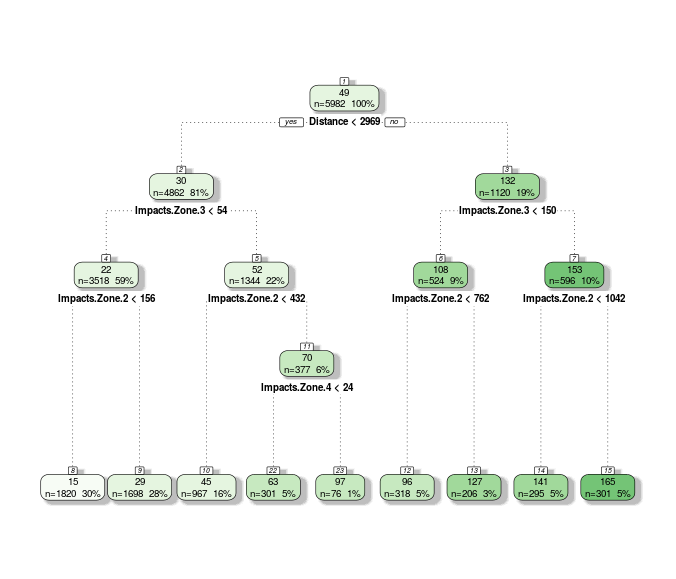
\includegraphics[width=12cm, height=9cm]{Images/DecisionTreeNoOut.png}
	\caption{The rattle package contains the FancyRPartPlot function which helps visualize the decision tree}
\end{figure}
\break\hfill

The numeric values at the top of each node display the predicted New.Bodyload value for the partition created by the node and the bottom values represent the number of observations in that partition and the proportion of observations in that partition. The condition surrounded by $yes$ and $no$ is the predictor and cutpoint that further partitions the predictor space into regions that maximizes the reduction in the residual sum of squares across all predictors. Zone variables dominate the model once the distance variable has partitioned the data. This makes sense as impacts are a source of acceleration and the tree suggests that high distances and high numbers of impacts lead to large values of New.Bodyload as outlined in 2.2.


\subsubsection{Clustering}
Plots of the variables that linear models found to be predictive of New.Bodyload seemed to all have a trend of being linear up to a certain point and then have a non-linear relationship beyond that point. This was motivation to implement a clustering algorithm on the data to explore if there was a natural split in the data. I decided to run a K-means clustering algorithm to explore mathematically if the data would be most efficiently partitioned in correspondence with the linear/non-linear trends observed in the data.  K-means clustering aims to partition n observations into k clusters in which each observation belongs to the cluster with the nearest mean, with the goal:
\[minimize \sum_{i=1}^{K}W(C_i)\]
The weight function W is defined using the sum of squared Euclidean distances between points by \[W(C_k)=\frac{1}{|C_k|}\sum_{i,j \in{C_k}}\sum_{l=1}^{p} (x_i^l-x_j^l)^2\]
where $C_i$ is the i$_{th}$ set in the partition and x$_i^l$ represents the $i_{th}$ observation of the $l_{th}$ variable. The intention was for the model to split the data into two groups, where models could be fit separately for each group. The clustering algorithm was ran with data limited to observations of variables found to be relevant from linear models, since it has already been concluded that those variables encode most of the signal and it is not desired to cluster around noisy variables. The results of the K-means clustering algorithm partitioned the data into sets of size 1125 and 4857 respectively. The centers of the variables in each of these sets are shown in figure 2.27. These results appear to add mathematical justification to the suspected non-linear nature of ``large" values observed in figures 2.28-2.33. The data could have been modeled using a piecewise linear function which fit the data in each group using a separate line, with the constraint that the lines had to meet at a knot point. This could have been explored further since the different groups resulting from the clustering seem to represent high volume/intensity training sessions vs. low volume/intensity sessions, (values of New.Bodyload could have different interpretations depending on the drills performed.)
\begin{figure}[h]
	\centering
	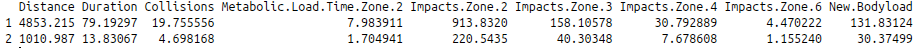
\includegraphics[width=16.8cm, height=1cm]{Images/ClusteringCenters.png}
	\caption{Centers of each K-Means Cluster}
\end{figure} 

\begin{figure}[h]
	\centering
	\begin{minipage}{.33\textwidth}
		\centering
		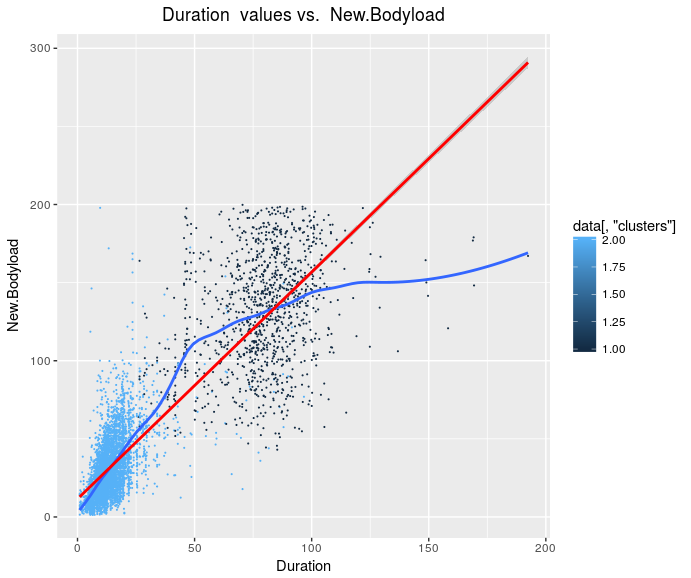
\includegraphics[width=\linewidth, height=6.5cm]{Images/DurationvsNBL.png}
		\captionsetup{width=.8\linewidth}
		\captionof{figure}{Duration vs. New.Bodyload clustered}
	\end{minipage}%
	\hfill
	\begin{minipage}{.33\textwidth}
		\centering
		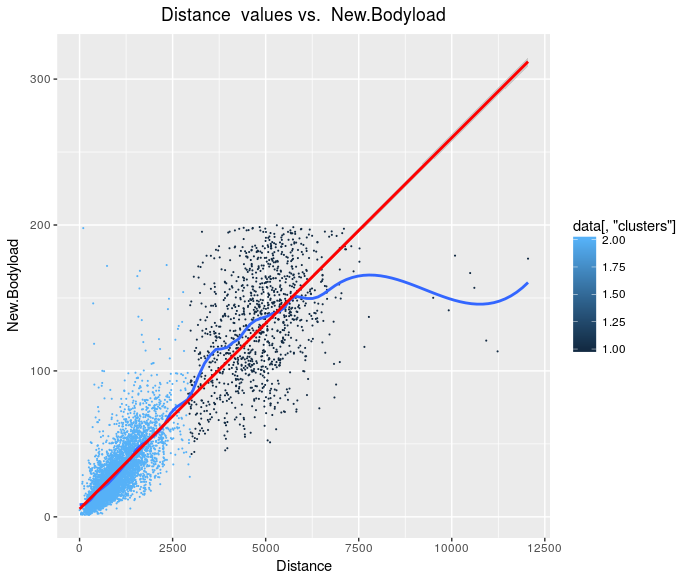
\includegraphics[width=\linewidth, height=6.5cm]{Images/DistancevsNBL.png}
		\captionsetup{width=.8\linewidth}
		\captionof{figure}{Distance vs. New.Bodyload clustered}
	\end{minipage} %
	\hfill
	\begin{minipage}{.33\textwidth}
		\centering
		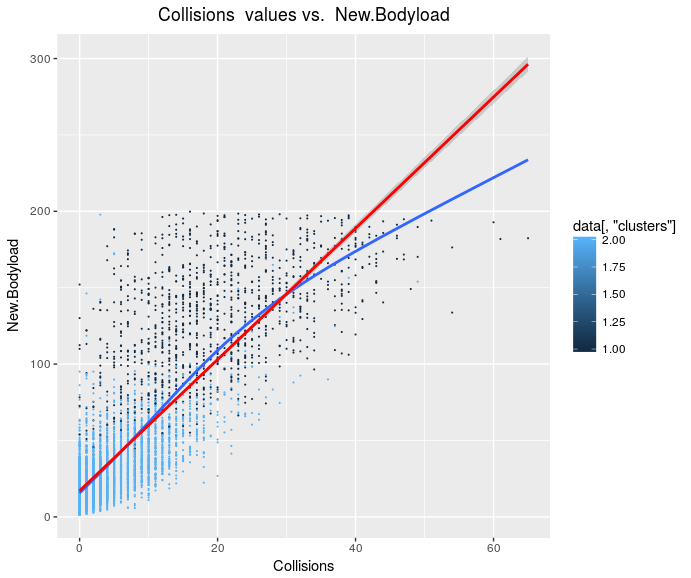
\includegraphics[width=\linewidth, height=6.5cm]{Images/CollisionsvsNBL.png}
		\captionsetup{width=.8\linewidth}
		\captionof{figure}{Collisions vs. New.Bodyload clustered}
	\end{minipage}
	\newline
	\centering
	\begin{minipage}{.33\textwidth}
		\centering
		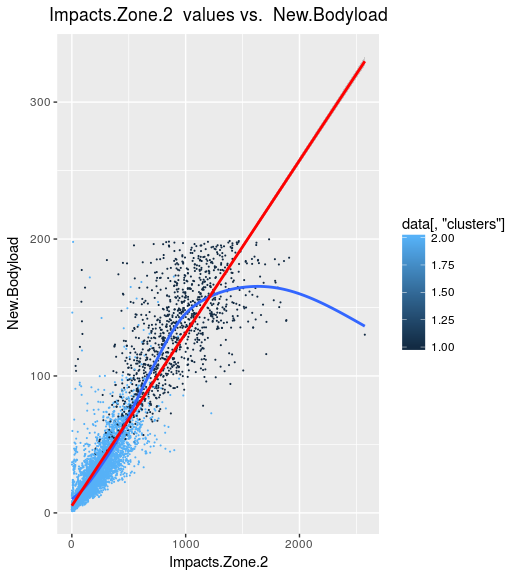
\includegraphics[width=\linewidth, height=6.5cm]{Images/ImpactsZone2vsNBL.png}
		\captionsetup{width=.8\linewidth}
		\captionof{figure}{Impacts.Zone.2 vs. New.Bodyload clustered}
	\end{minipage}%
	\hfill
	\begin{minipage}{.33\textwidth}
		\centering
		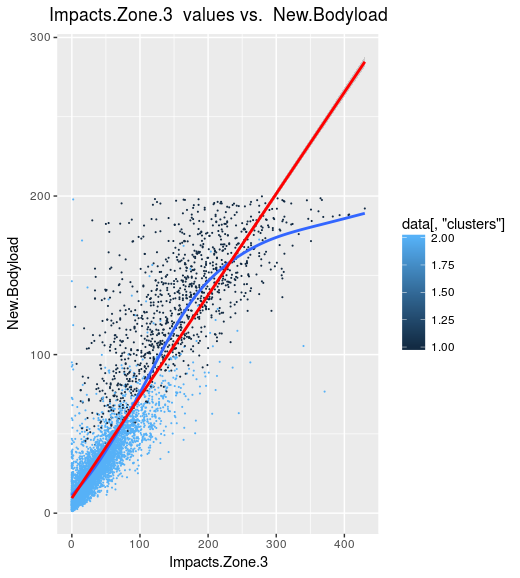
\includegraphics[width=\linewidth, height=6.5cm]{Images/ImpactsZone3vsNBL.png}
		\captionsetup{width=.8\linewidth}
		\captionof{figure}{Impacts.Zone.3 vs. New.Bodyload clustered}
	\end{minipage} %
	\hfill
	\begin{minipage}{.33\textwidth}
		\centering
		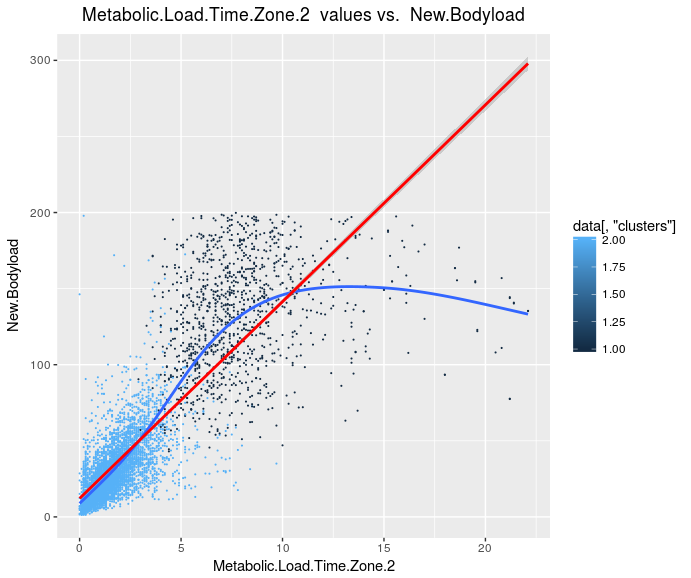
\includegraphics[width=\linewidth, height=6.5cm]{Images/MetLoad2vsNBL.png}
		\captionsetup{width=.95\linewidth}
		\captionof{figure}{Metabolic.Load.Time.Zone.2 vs. New.Bodyload clustered}
	\end{minipage}
\end{figure}
\break\hfill

\subsubsection{K Nearest Neighbors Regression (KNN)}
The K Nearest Neighbors algorithm is an example of a non-parametric algorithm. The consequence of this is that the algorithm doesn't make any assumptions about the nature of the data and so the results of the model won't suffer from some of the symptoms that plagued the linear models. The algorithm was developed as a direct approximation of the function that minimizes the Expected Prediction Error:
\[EPE(f)=E(Y-f(X)^2) = E_XE_{Y|X}((Y-f(X))^2|X)\]
Since X has been fixed, it is not longer a random variable and so it suffices to minimize this function point-wise using basic calculus, letting c=f(x) \cite{ESL}: 
\[argmin_c \int\int((Y-c)^2 f_{Y|X}(y)dy)f_X(x)dx=\] the value of c such that: \[\frac{d}{dc}\int (Y-c)^2f_{Y|X}(y)dy=0\]\[\frac{d}{dc}(
\int Y^2f_{Y|X}(y)dy -2c\int Yf_{Y|X}(y)dy+c^2\int f_{Y|X}(y)dy)=
\frac{d}{dc}(E[{Y^2}|X]-2cE[Y|X]+c^2)=0\]
\[f(x)=c=E[Y|X]\]
The K Nearest Neighbor algorithm offers an approximation of this: 
\[\hat{f}(x)=Ave(y_i|x_i \in N_k(x))=\frac{1}{k}\sum_{x_i\in N_k(x)}^{} y_i \]
where expectation of the response is approximated by averaging the response value of the nearest k points to x. This relies on the assumption of the points $x_i \in N_k(x)$ being ``close" to the value of x, which is not true of every data set. Typically the KNN regression algorithm will use a weighted average where the response value of each of the $x_i \in N_k(x)$ is first weighted by the inverse of its Euclidean distance to the predicted data point and then averaged. KNN can be used to make inferences from the data depending on the value of k that optimizes the MSE of the data.\hfill\break
\begin{wrapfigure}{r}{5cm}
	\vspace{-2.2em}
	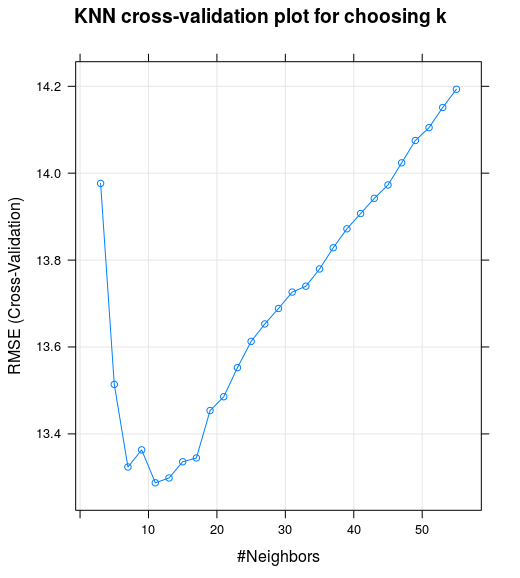
\includegraphics[height=5cm,width=5.2cm]{Images/KNNCrossValidation.png}
	\caption{Choice of k should be 11 based on cross-validation}
\end{wrapfigure}
A small value of k means that noise will have a higher influence on the result, i.e. the model will have a higher ratio of variance to bias compared to a model that uses a relatively large value of k. The KNN model offers a non-parametric comparison to the parametric linear models, where the parametric approach will outperform the nonparametric approach if the parametric form that has been selected is close to the true form of f(x) \cite{ISLR}. The optimal value of k was chosen using cross validation as shown in Figure 2.34.
\hfill\break

\subsection{Modeling data with suspected outliers}
The data including suspected outliers was modeled in a very similar fashion to the data excluding suspected outliers. The statistical modeling file can be found at \cite{ModellingWithoutOutliers}. The results of these models are shown in Table 2.2. The outliers had a significant effect on the modeling of the data, with performance metrics suggesting that the outliers may have been erroneous/miscalibrated measurements. Most noticeable is the fact that the test set mean squared error value was approximately half that of the train set error for most of the models constructed, which suggests that either the data was not split randomly or that there were a few outlying values in the training set that accounted for a large proportion of the MSE observed in the training set. A boxplot of the distribution of values of New.Bodyload reveal that there were significantly more large values of New.Bodyload in the training data set than the testing data set. The models struggled to predict these large values of New.Bodyload which lead to large values of MSE for both the train and test sets. The residual plot in figure 2.37 has a spline fitted to show the wildly inaccurate predictions for large values of New.Bodyload. The results table shows that every linear model struggled to predict large values of New.Bodyload, however the non-linear models also struggled. The optimum value of k=51 for KNN suggests that the model was essentially predicting in a similar manner to the Null Model, where the value of the response was optimised by averaging over a large region.

\begin{figure}[h]
	\centering
	\begin{minipage}{.33\textwidth}
		\centering
		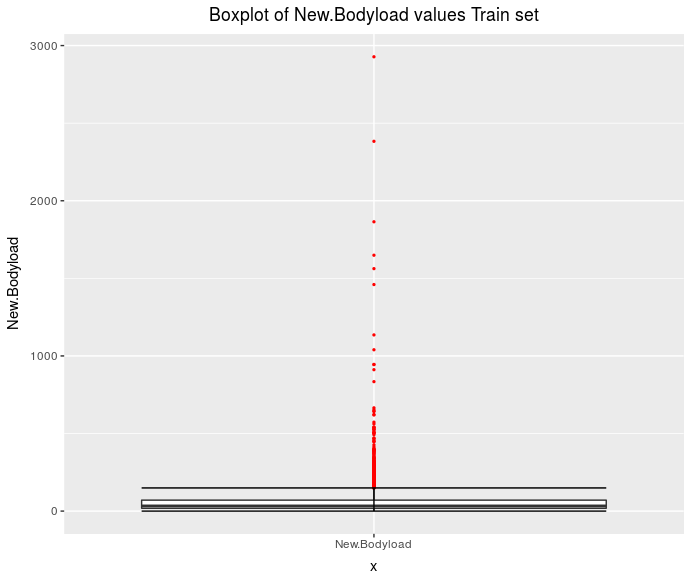
\includegraphics[width=\linewidth, height=6.5cm]{Images/NBLDistributionTrain.png}
		\captionsetup{width=.8\linewidth}
		\captionof{figure}{}
	\end{minipage}%
	\hfill
	\begin{minipage}{.33\textwidth}
		\centering
		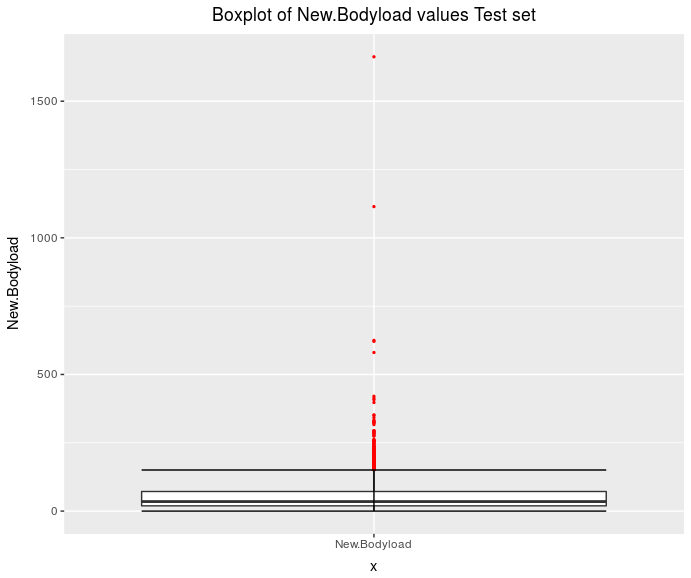
\includegraphics[width=\linewidth, height=6.5cm]{Images/NBLDistributionTest.png}
		\captionsetup{width=.8\linewidth}
		\captionof{figure}{}
	\end{minipage} %
	\hfill
	\begin{minipage}{.33\textwidth}
		\centering
		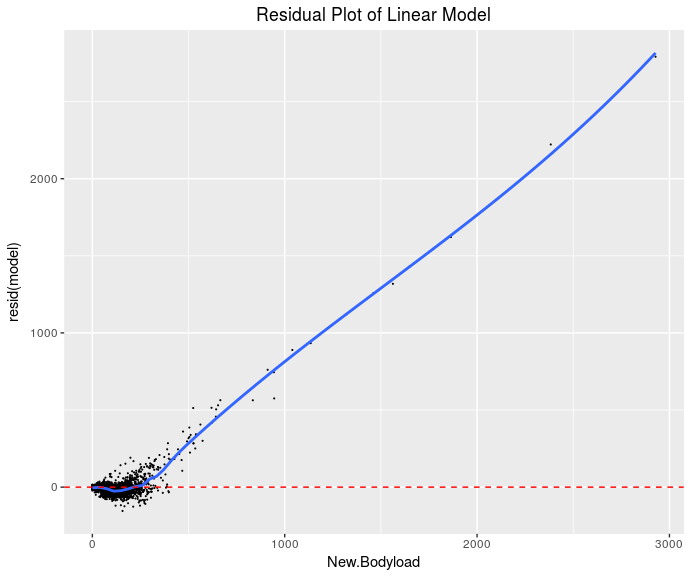
\includegraphics[width=\linewidth, height=6.5cm]{Images/LinearModelResidualWithOutliers.png}
		\caption{Residual Plot of Simple Linear Regression}
	\end{minipage} %
\end{figure} 
The discrepancies between corresponding models in the two sets of analyses suggest that using the techniques explored in this project, it is possible to predict values of New.Bodyload when New.Bodyload is ``small" (less that approximately 200) but values of New.Bodyload that are ``large" (greater than approximately 200) cannot be predicted with a reasonable degree of accuracy. The implications of this are that either the data provided was not sufficient to provide the motivating factors of the large values, the statistical models that were constructed were too simplistic, or that these values were indeed outliers and they should have been treated as erroneous measurements. Since the data provided could not give enough information on whether the large values of New.Bodyload were outliers or not, it was difficult to determine which of these cases was the most likely scenario. Further discussion of this is provided in the conclusion.
\section{Results}
\def\arraystretch{1.5}%
\begin{table}
	\centering
	\begin{tabular}{|p{6.2cm}||p{2cm}|p{2cm}|p{2cm}|p{2.57cm}|}
		\hline
		\multicolumn{5}{|c|}{Analysis Without Suspected Outliers} \\
		\hline
		\textbf{\footnotesize Model Name} & \textbf{\footnotesize Train set Adjusted $R^2$} &\textbf{\footnotesize Train set MSE} & \textbf{\footnotesize Test Set MSE} & \textbf{\footnotesize No. Variables / Tuning Parameter}\\
		\hline
		Null Model (Intercept) & 0 & 2142.12 & 2091.22 & 0\\
		\hline
		Simple Linear Regression & 0.955 & 96.88 & 110.41 & 43\\
		\hline
		Forward Stepwise Regression & 0.828 & 369.13 & 380.78 & 1\\
		\hline
		Forward Stepwise Regression & 0.902 & 210.56 & 231.54 & 2\\
		\hline
		Forward Stepwise Regression & 0.926 & 157.64 & 167.96 & 3\\
		\hline
		Forward Stepwise Regression & 0.935 & 138.34 & 153.67 & 4\\
		\hline
		Forward Stepwise Regression & 0.940 & 127.75 & 143.41 & 5\\
		\hline
		Forward Stepwise Regression & 0.948 & 112.38 & 128.36 & 6\\
		\hline
		Best Subset Selection & 0.906 & 202.28 & 205.86 & 2\\
		\hline
		Best Subset Selection & 0.929 & 151.28 & 160.54 & 3\\
		\hline
		Best Subset Selection & 0.938 & 133.74 & 142.60 & 4\\
		\hline
		Best Subset Selection & 0.946 & 115.51 & 129.41 & 5\\
		\hline
		Best Subset Selection & 0.951 & 105.58 & 119.07 & 6\\
		\hline
		Best Subset Selection & 0.951 & 103.08 & 116.94 & 7\\
		\hline
		Polynomial Regression & 0.962 & 77.92 & 159.69 & 338\\
		\hline
		Polynomial Regression & 0.939 & 133.74 & 142.60 & 3\\
		\hline
		Lasso Regression & 0.954 & 97.14 & 110.72 & 41/$\lambda=0.0187$\\
		\hline
		Regression with Interaction Terms & 0.946 & 114.87 & 130.94 & 5\\
		\hline
		Principal Components Regression  & 0.929 & 152.26 & 170.54 & 9\\
		\hline
		Partial Least Squares Regression & 0.949 & 109.89 & 120.57 & 12\\
		\hline
		Regression Tree & 0.895 & 223.49 & 268.42 & 20\\
		\hline
		KNN & 0.852 & 317.00 & 410.64 & k=11\\
		\hline
	\end{tabular}
	\caption{Results of modeling the data excluding suspected outliers}
\end{table}
\def\arraystretch{1.5}%
\begin{table}
	\centering
	\begin{tabular}{|p{6.2cm}||p{2cm}|p{2cm}|p{2cm}|p{2.57cm}|}
		\hline
		\multicolumn{5}{|c|}{Analysis With Suspected Outliers} \\
		\hline
			\textbf{\footnotesize Model Name} & \textbf{\footnotesize Train set Adjusted $R^2$} &\textbf{\footnotesize Train set MSE} & \textbf{\footnotesize Test Set MSE} & \textbf{\footnotesize No. Variables / Tuning Parameter}\\
			\hline
		Null Model (Intercept) & 0 & 9482.28 & 6974.72 & 0\\
		\hline
		Simple Linear Regression & 0.486 & 4841.31 & 2721.21 & 43\\
		\hline
		Forward Stepwise Regression & 0.428 & 5427.87 & 3278.35 & 1\\
		\hline
		Forward Stepwise Regression & 0.463 & 5094.95 & 2924.50 & 2\\
		\hline
		Forward Stepwise Regression & 0.474 & 4981.80 & 2722.23 & 3\\
		\hline
		Forward Stepwise Regression & 0.478 & 4947.71 & 2712.14 & 4\\
		\hline
		Forward Stepwise Regression & 0.480 & 4930.59 & 2690.39 & 5\\
		\hline
		Forward Stepwise Regression & 0.481 & 4919.26 & 2692.87 & 6\\
		\hline
		Best Subset Selection & 0.463 & 5094.95 & 2924.50 & 2\\
		\hline
		Best Subset Selection & 0.474 & 4981.800 & 2722.23 & 3\\
		\hline
		Best Subset Selection & 0.478  & 4947.42 & 2708.63 & 4\\
		\hline
		Best Subset Selection & 0.480 & 4929.60 & 2684.68 & 5\\
		\hline
		Best Subset Selection & 0.481 & 4915.57 & 2682.85 & 6\\
		\hline
		Best Subset Selection & 0.482 & 4906.75 & 2690.189 & 7\\
		\hline
		Polynomial Regression & 0.515 & 4366.21 & 3246.28 & 337\\
		\hline
		Polynomial Regression & 0.491 & 4912.04 & 2673.81 & 7\\
		\hline
		Lasso Regression & 0.483 & 4902.81 & 2706.15 & 15/$\lambda$=1.279\\
		\hline
		Regression with Interaction Terms & 0.480 & 4929.60 & 2684.68 & 5\\
		\hline
		Principal Components Regression & 0.469 & 5038.63 & 2838.00 & 9\\
		\hline
		Partial Least Squares Regression & 0.484 & 4895.695 & 2691.12 & 12\\
		\hline
		Regression Tree & 0.549 & 4254.844 & 2854.84 & 28\\
		\hline
		KNN & 0.450 & 5212.703 & 3625.64 & k=51\\
		\hline
	\end{tabular}
	\caption{Results of modeling the data including suspected outliers}
\end{table}
\break\hfill

\section{Conclusions}
\subsubsection{Suspected Outliers}
The first question addressed is whether the analyses have indicated that the anomalous looking values of New.Bodyload were in fact outliers. Based on the results of the exploration of the data and the analyses, there seem to be three realistic explanations for the largest observed values of New.Bodyload: 
\begin{enumerate}
	\item \emph{Some GPS units were miscalibrated}. As noted in section 2.2, the New.Bodyload variable is constructed by essentially aggregating the scaled and normalized values of the magnitude of the acceleration vector over a period of time. The scaling of the variable is dependent on exercise factor, which suggests that if an incorrect value of exercise factor was used then some values of New.Bodyload would be incorrectly scaled and therefore very large or small in relation to the others. Since one data point was removed due to an obvious miscalibration of the GPS unit, this seems like a realistic scenario.
	
	\item \emph{Some variable that was not provided held key information.} It could be the case that there simply weren't enough variables in the data to fully explain the trends associated with New.Bodyload. For example, if the acceleration zones were more granular, then it might be observed that very high values of New.Bodyload resulted from extreme values of acceleration. This could indicate that the data points were in fact outliers if the acceleration values were very high (which could indicate that the GPS units were accidentally dropped, for example.) Again, the construction of New.Bodyload reveals that this could be a realistic scenario as the variable accumulates at a rate of O($NV^3$), indicating that one large acceleration could result in a correspondingly large value of New.Bodyload.
	
	\item \emph{The statistical models were not sophisticated enough to detect trends.} It could be the case that a transformation of the dependent variable and a more complex statistical model trained on the data set including suspected outliers could have yielded more predictive models which could have explained why the relatively large values of New.Bodyload were observed. This was not explored fully in the analysis but a model that had a weighted loss function designed to penalize large residuals in a different proportion to small residuals could detect possible motivating factors behind the large values of New.Bodyload. This scenario is the most unlikely, as even when flexible piecewise linear and non-linear models were briefly explored, the models struggled to detect a trend in large values of New.Bodyload.
\end{enumerate}
There is no conclusive evidence to deem the suspected outliers as true outliers or not. The project could have been extended to explore these values further.

\subsubsection{Optimal Models}
The models that were most interpretable and also explained the variance observed in New.Bodyload well were the best subset selection model limited to 7 predictors and the linear model involving interaction terms limited to 5 predictors for the both analyses. As seen in table 2.1, many of the models had comparable mean squared errors, but as discussed in section 2.3, linear models with few variables that fit the data well are most valuable for making inferences. The lowest MSE achieved on the test set was 110.41 (2673.81 test set). The best subset selection models with 7 variables achieved a test set MSE of 116.94 (4906.75 with suspected outliers) with an adjusted $R^2$ of 0.951 (0.482 with suspected outliers) and the interaction model with 5 variables achieved a test set MSE of 130.94 (2684.68 with suspected outliers). These models were successful in reducing the dimensionality of the data from 43 variables to \textless7 while simultaneously retaining most of the variability in the data. Given more time, an extension of these models could be fit piecewise to the clusters described in fig 2.28-2.33.

\subsubsection{Inferences}
Since the data including outliers could not be modeled effectively, it makes sense to mostly discuss the results of the modeling of the data excluding suspected outliers. The variables that appeared in the best subset selection model limited to 7 variables were Duration, Impacts.Zone.2, Impacts.Zone.3, Impacts.Zone.4, Impacts.Zone.6, Collisions and\break Metabolic.Load.Time.Zone.2. The model summary is shown in Figure 2.38. The model is essentially stating that New.Bodyload is predicted by the formula:

\hfill
\newline
$
0.384\pm{0.195}+Duration(0.239\pm{0.010})+Impacts.Zone.2(0.035\pm{0.001})+Impacts.Zone.3(0.174\pm{0.006})+Impacts.Zone.4(0.258\pm{0.021})+Impacts.Zone.6(1.719\pm{0.063})+Collisions(0.640\pm{0.028})+Metabolic.Load.Time.Zone.2(3.021\pm{0.094})
$
\hfill
\newline

The interpretation of this is that taking all variables as being fixed but one, e.g. Collisions, then every additional collision would result in New.Bodyload increasing by 0.640$\pm{0.028}$. This model implies that the quantity and magnitude of impacts experienced, the duration of the training session and the metabolic load experienced by the athlete during the drill are the most important factors in determining the associated value of New.Bodyload, which agrees with the construction of the variable outlined in 2.2. Note that the intercept of the model, 0.384, is close to zero, which indicates that when all variables are fixed at zero, the value of New.Bodyload will be close to zero, which agrees with the documentation. The interaction model can be viewed analogously, with the variables Impacts.Zone.2, Impacts.Zone.3, Impacts.Zone.6, Metabolic.Load.Time.Zone.2 and Duration*Collisions deemed the best combination of predictors. New.Bodyload is predicted by:

\hfill
\newline
$3.677\pm{0.219}+Impacts.Zone.2(0.033\pm{0.001})+Impacts.Zone.3(0.243\pm{0.004})+\break Impacts.Zone.6(2.278\pm{0.059})+Metabolic.Load.Time.Zone.2(3.842\pm{0.089})+Duration*Collisions(0.011\pm{0.0003})
$

\hfill
\newline
Both models are similar in terms of the variables included and the values of their coefficients, which was true of most of the models constructed. A comparison of the variance inflation factors in these models shows that the variables used in both models exhibited multicollinearity, but to a much lesser degree than that of models using more variables.

 \begin{figure}[h]
 	\centering
 	\begin{minipage}{.45\textwidth}
 		\centering
 		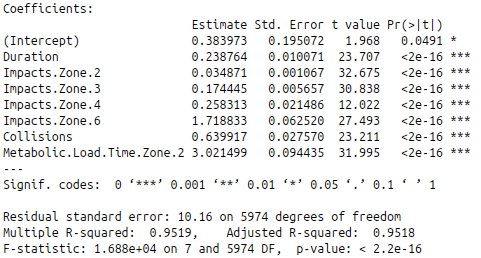
\includegraphics[width=\linewidth, height=4.2cm]{Images/BestSubsetSelectionConclusion.png}
 		\captionof{figure}{Summary of Best Subset Selection Model}
 	\end{minipage}%
 	\hfill
 	\begin{minipage}{.45\textwidth}
 		\centering
 		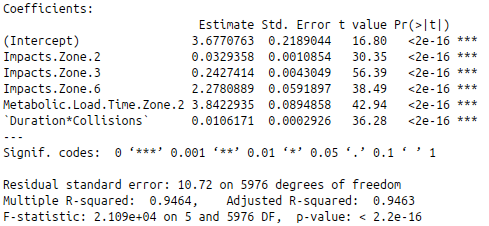
\includegraphics[width=\linewidth, height=4.2cm]{Images/InteractionModelConclusion.png}
 		\captionof{figure}{Summary of Interaction Model}
 	\end{minipage} 
 \end{figure}
\subsubsection{Further Exploration and Analyses}
This project was limited by time and so there is large scope for further analysis. Regarding New.Bodyload, further investigation using clustering techniques and piecewise models could have yielded more insightful information regarding its construction. The analysis could also have been carried out using a different intercept for each athlete, or by predicting New.Bodyload divided by Duration. It is worth noting that New.Bodyload is an example of a compound Poisson process, where the i$_{th}$ value of New.Bodyload in the data is given by
\[BL_i=\frac{1}{100}\sum_{j=1}^{N(t)} \frac{{(NV_{ij}+NV_{ij}^3)}}{EF_i} \]
where $NV_{ij}$ denotes the j$_{th}$ observed value of the normalized acceleration magnitude greater than 0.25g in the time period t for $i_{th}$ entry in the data set and $EF_i$ denotes the exercise factor associated with the $i_{th}$ entry in the data set. N(t) should approximately follow a Poisson distribution, where the arrival rate $\lambda$ is fixed, the probability that two normalized acceleration magnitudes that are greater than 0.25g occur in $\Delta$t should be small compared to just one (due to the sampling frequency) and the event of any arrival occurring should be independent of all other arrivals. These assumptions are somewhat relaxed in this case. 
\hfill\break
\newline
By regressing $bl_i$ (the i$_{th}$ observation of New.Bodyload in the data set) on the $x_{ip}$ predictor variables associated with the $i_{th}$ observation, an estimate can be obtained for the mean response $\hat f(x)=E[BL|X]$ at any given combination of values $x_{i1}, x_{i2}, ... , x_{ip}$ of the input variables $X_{i1}, X_{i2}, ... , X_{ip}$. Using the least squares estimator, this is given by $\hat{bl_i} = \hat{\beta{_0}}+\sum_{i=1}^{p}\hat{\beta}_ix_i$. A confidence interval for this estimator is desired for this predictor. Denoting $\frac{{(NV_{ij}+NV_{ij}^3)}}{EF_i}$ as $U_{ij}$ and assuming $U_{i1}$, $U_{i2}$, ... , $U_{in}$ are I.I.D., then Wald's theorem shows that 
\[E[Y_i]=E[\sum_{j=1}^{N(t)}U_{ij}]=E[N(t)]E[U_i]\]
and 
\[Var[Y_i]=Var[\sum_{j=1}^{N(t)}U_{ij}]=Var[N(t)]E[U_i^2]\]
where $U_i$ is any one of the $U_{ij}$ and $Var[N(t)]=E[N(t)]=\lambda t$, where $\lambda$ is the arrival rate of the Poisson variable N(t). Since the $Y_i$ are not identically distributed, assuming a lack of independence, an approximation to both $E[Y_i]$ and $Var[Y_i]$ can be tediously derived using an analogue of Wald's theorem and the delta method (to account for the fact that $U_{ij}$ is a ratio of random variables). One can then derive an asymptotic  distribution of an appropriately standardized version of $\hat Y_i\approx E[Y|X=x_i]$ and from this a confidence interval of $E[Y|X_i]$ is routine to find. Note that a simplified version of the formula is obtained in the special case when the denominator $EF_i$ of $U_i$ is independent of i. The details of the derivation are omitted but this could be explored further to extend inferences developed in the project.



	
	\newpage
	\chapter{Data Visualization}
	Having completed the statistical analysis of the data, a natural question arises: how is it possible to convey the results observed in the analysis to coaches and athletes so that they can obtain an understanding of the data that they have collected? Visualization is an important part of any data analysis as it can offer rapid and meaningful insight into the data due to the inherent human dependency on vision for interpretation. Typically datasets will have multiple dimensions and facets, so in order to gain a broad insight into the data, multiple graphs and images are necessary. Any data visualizations will ideally be portable, system independent and reusable. The options explored for constructing such a system were:
\begin{enumerate}
	\item Building a web application using well-established web development tools such as Ruby on Rails, or Django. This option was not implemented as it would require extensive quantities of boilerplate code.
	\item Creating an executable program that can be run locally. This had a drawback in that the system would somehow need to be distributed, which went beyond the scope of this project.
	\item Building a web application using a customized web framework such as Spyre or Shiny. Shiny is a package within R, an open source statistical language and development framework, that facilitates the development of reactive data visualizations through a web browser. This was the most attractive choice of the three. Since the data analysis was performed using R, Shiny was chosen to develop the application.
\end{enumerate}

\section{Shiny}
Shiny is an open source R package that provides a high level web development framework. Shiny was developed with the aim of converting analyses into interactive web applications with minimal knowledge of HTML, CSS, Javascript and other common web-development languages. The focus is on presenting graphics to the end user which can enlighten them about their data. The advantages of using Shiny are:
\begin{itemize}
	\item It's interactive which means it can offer a dynamic user experience. 
	\item Shiny applications are written in R and can utilize all of the libraries that are already available in the R language.
	\item The development of a shiny App is centered around displaying graphics generated with R to the user. If you can program with R, you can program with Shiny.
\end{itemize}
Since R was used to perform the statistical analysis, it was a natural extension to develop the visualizations using the Shiny package. Every Shiny application consists of a minimum of a server function and a user interface function which follows the ``separation of concerns" design principle. The server is concerned with data manipulation and mapping user inputs to various types of output, whereas the user interface is concerned with data presentation. I followed the convention in Shiny of creating a project folder and then writing R files named server.r, ui.r and a www folder which contains css and image files used by the browser in the App, found at \cite{ShinyServer}\cite{ShinyUI}.

\section{Functionality}
In the application that I developed, I set out a certain amount of functionality that would be necessary to make the App straightforward for the user to operate. The following subsections offer an exposition of how this was achieved.

\subsection{Dropbox File Upload}
It was necessary for  the App to allow the user to upload their own csv file in order to display their data. This was easily be achieved through using a local file uploader, which Shiny provides using the fileInput widget. However, only facilitating local file uploads imposed limitations: it is undesirable for a sports team's data to be located on a number of different machines rather than on a central repository, the most obvious consequence being that if one of the machines is damaged, data could be lost permanently. For these reasons, tools like Dropbox are often used to store and access athlete data. I decided to add the option to upload data from the users' Dropbox account to the App. This required using the package rdrop2 to facilitate the user logging into their dropbox and permitting the App to upload data from their dropbox to the App. This was achieved using the following code segment:

\begin{lstlisting}[language=R, basicstyle=\tiny]
dropboxDown=reactive({
  if(input$dropboxDownload){
  #only run this authorization once (not sure how to do this without the use of global variable)
    if(!alreadyVisited){
      #consider adding new_user=TRUE
      dropbox_credentials=drop_auth(cache=FALSE)
      updateCheckboxInput(session, "dropboxDownload",label='Choose a file:')
      #update file choices
	  updateSelectizeInput(session,'dropboxFileSelection',choices=basename(
	  drop_search('.csv')[order(drop_search('.csv')$modified),]$path))
	  #set global alreadyVisited variable to TRUE as this behaviour should only occur once
	  alreadyVisited<<-TRUE
	}
	#update the input file to the file selected by the user
	inFile1=input$dropboxFileSelection
	#check file exists
	if (is.null(inFile1)){
	  print('No file provided')
	  return(NULL)
	}
	else{
	  #can deal with RData and csv formatted files
	  if(length(grep('.csv',inFile1))!=0){
	    #read csv by finding the path in dropbox, ensure ProcessedData is global
	    ProcessedData<<-drop_read_csv(drop_search('.csv')[match(inFile1,basename(
	    drop_search('.csv')$path)),]$path,stringsAsFactors=FALSE)
	    #be careful as write.csv adds an x column if column.names=FALSE
	    ProcessedData$Date=as.Date(ProcessedData$Date)
	  }
	  else if(length(grep('.RData',inFile1))!=0){
	    load(inFile1$datapath)
	    ProcessedData<<-ProcessedData
	  }
    }
    if(exists('ProcessedData')){
	  #If the data exists, preprocess it
      Preprocess()
      #now allow the user to download a report
      shinyjs::enable("report")
      shinyjs::enable("refreshReport")
      #call data preprocessing function, look into passing Preprocess to this function
    }
  }
})
\end{lstlisting}
This led the user through the sequence of events displayed in figures 3.1-3.4: 
\begin{figure}[h]
	\centering
	\begin{minipage}{.48\textwidth}
		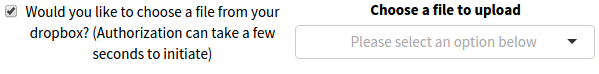
\includegraphics[width=1\linewidth, height=1cm,left]{Images/RDropCheckbox.png}
		\caption{1). Click checkbox}
	\end{minipage} %
	\hfill
	\begin{minipage}{.4\textwidth}
		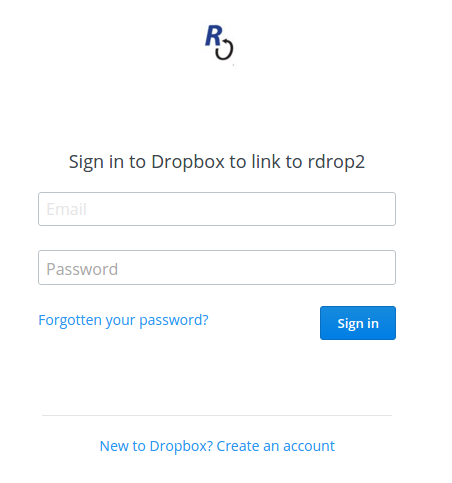
\includegraphics[width=0.9\linewidth, height=3cm,right]{Images/RDropLogin.png}
		\caption{2). Sign in to Dropbox}
	\end{minipage} %
	\newline
	\centering
	\begin{minipage}{.45\textwidth}
		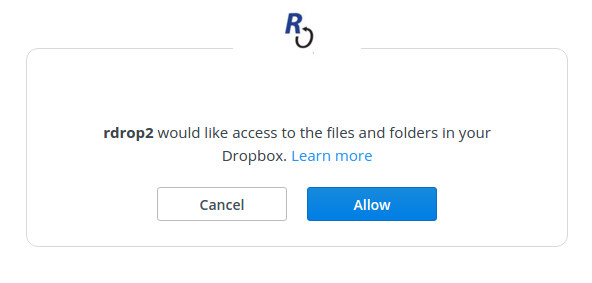
\includegraphics[width=1\linewidth, height=3cm,left]{Images/RDropAuth.png}
		\caption{3). Authorize file access}
	\end{minipage} %
	\hfill
	\begin{minipage}{.45\textwidth}
		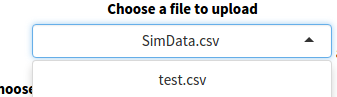
\includegraphics[width=1\linewidth, height=2cm,right]{Images/rdropDropDown.png}
		\caption{4). Upload Dropbox file}
	\end{minipage}
\end{figure}

\break\hfill

The rDrop2 package stores tokens containing the users password and user name so that the user does not have to log in every time the App is used, however this caused security issues regarding the safe storage of these details. There are options in the function drop\_auth which prevented the caching of login details by the application and also the option of specifying whether a new user is logging in (and whether previously cached details should be overwritten). In practice however, it seemed that the application created a file named .httr-oauth containing the cached user login information regardless of these options. This would be a major issue if the code was used in production but since the application was proof of concept, it was not resolved.

\subsection{CSV Upload Format}
The user must upload the data in a certain file format for this application to be able to process the file. From the outset I intended to write an application that would impose a minimum amount of restrictions on the user with the intent of having a scalable and extendable program. The modularity of the code has the consequence of decoupling the displays from the variables that are being displayed. In the application functions took as input the name of any numeric column in the data and outputted graphs. This meant that the only variables that must necessarily be present in the data are Date and Name (of athlete). The consequence of this is that the application can be modified in a matter of minutes to display the same graphs and summaries for a csv file containing any type of numeric Athlete data. 

\subsection{Application Tabs}
The rest of the functionality of the application was modularized into tabs which could be navigated in order to display a specific plot or summary.
\newpage
\subsubsection{Longitudinal Plot}
\begin{wrapfigure}{r}{9cm}
	\vspace{-2em}
	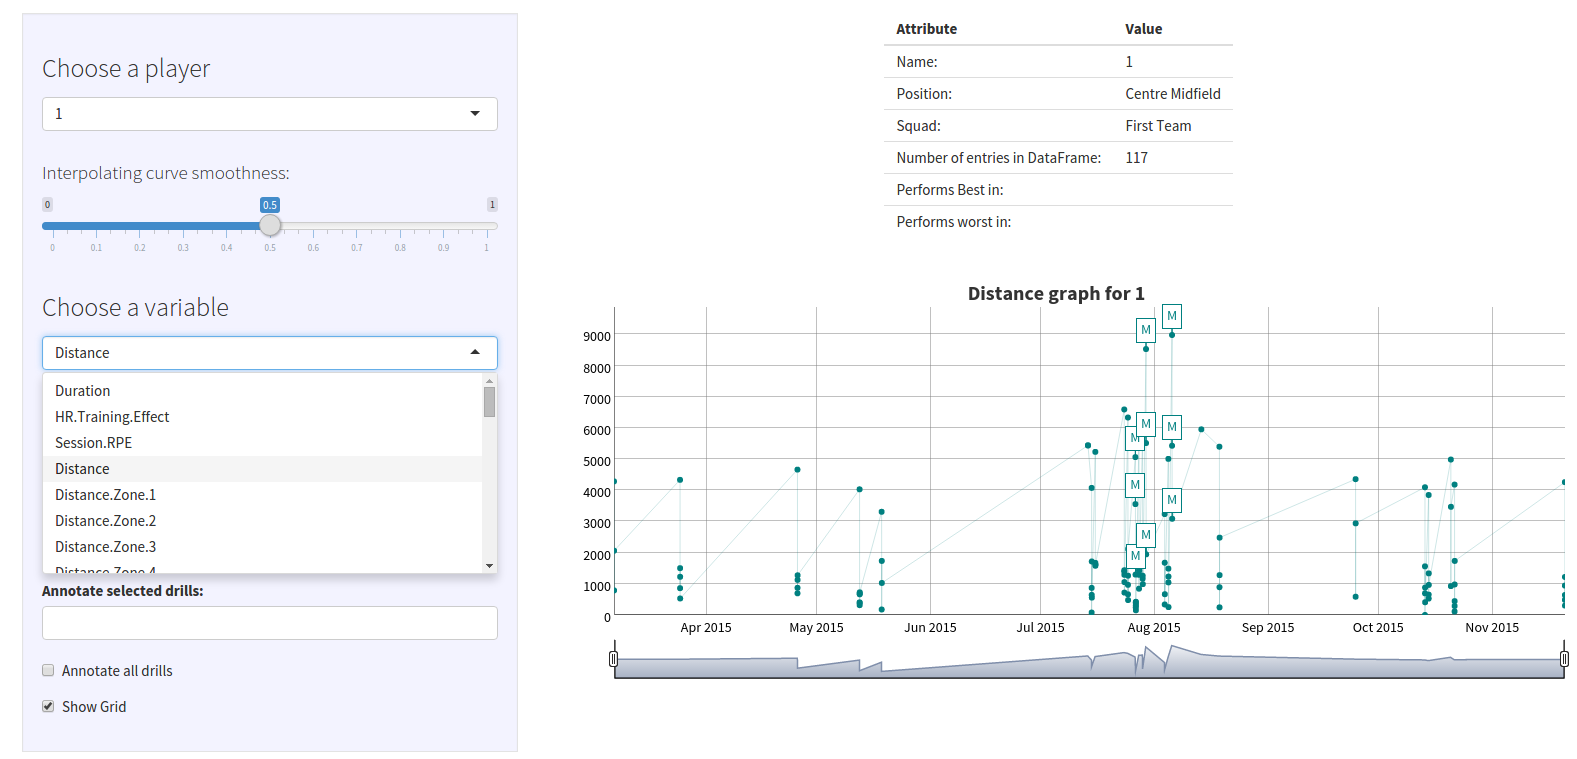
\includegraphics[height=5cm, width=10cm]{Images/PlotTab.png}
	\caption{Longitudinal Plot Tab}
\end{wrapfigure}
The tab that the application navigates to by default displays a longitudinal plot. This plot gives the user graphical information about how some aspect of the athletes' training has changed over time. The user can subset the graph to a certain date range and has the option to compare another athlete on the same graph. The option is also given to annotate drills so that if there is an unusual looking data point, the application user can immediately figure out which training session the unusual data originated from. The R dygraph package was the main tool used to achieve this. 

\subsubsection{Training Calendar}
\begin{wrapfigure}{r}{9cm}
	\vspace{-2em}
	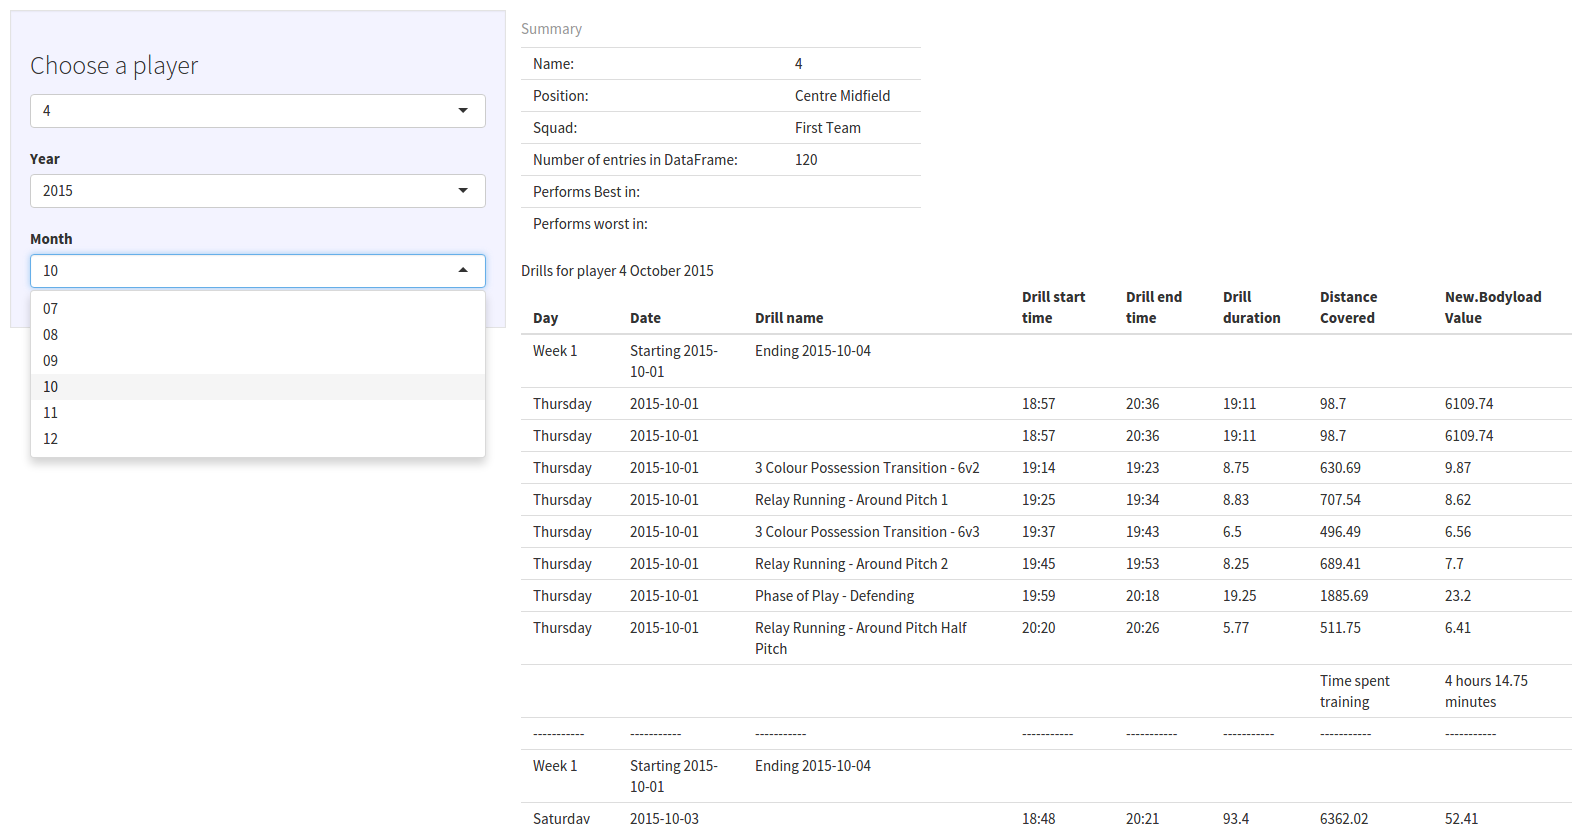
\includegraphics[height=5cm, width=10cm]{Images/TrainingCalendarTab.png}
	\caption{Training Calendar tab}
\end{wrapfigure}
The training calendar tab provides the user with a readable account of an individual athlete's training schedule over a month in the data provided. The calendar displays which drills the athlete performed, the drill start and end times, the total duration of the drill, the distance that the player covered in the drill as well as the New.Bodyload value generated for that drill. The calendar is broken into weeks of the month so that athletes and coaches have a week-by-week account of the drills that were performed. The code was written so more details about the training session can be conveniently added.


\subsubsection{Bar Plot}
\begin{wrapfigure}{r}{9cm}
	\vspace{-2em}
	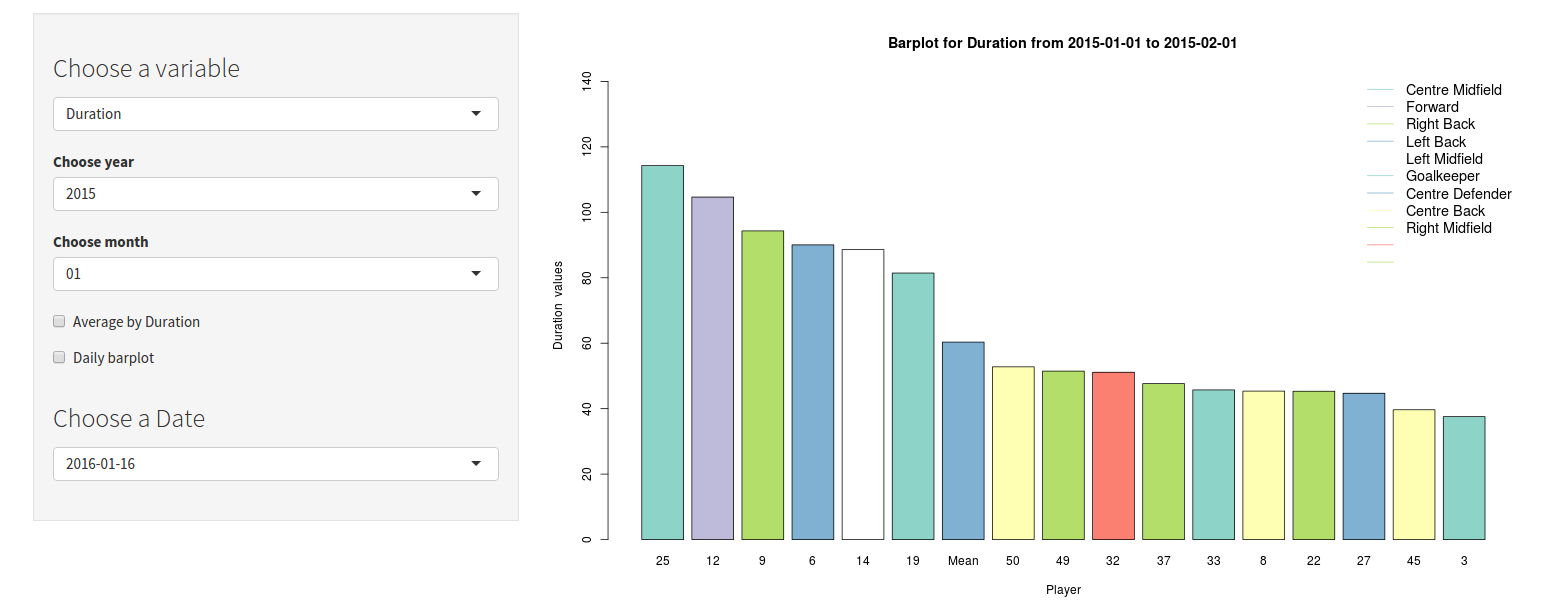
\includegraphics[height=5cm, width=10cm]{Images/BarplotTab.png}
	\caption{Bar Plot tab}
\end{wrapfigure}
The bar plot tab was designed to give a graphical representation of how players in the team performed relative to each other over a date range for a certain variable. This is useful as sometimes absolute figures can lose meaning whereas comparing each player in the team to other players in the team quickly informs coaches who is under performing in certain aspects. The bar plot is coloured by position so that it is easy to compare players competing for the same position. There is an option to average the displayed variable by duration because, as discussed in 2.2.2, accumulative variables are not measured according to the same scale when mean values are taken. Therefore this plot can be somewhat misleading and should be used with caution. There is also an option to view the data with greater granularity by selecting to display the bar plot over an individual date.

\subsubsection{Rankings}
\begin{wrapfigure}{r}{9cm}
	\vspace{-2em}
	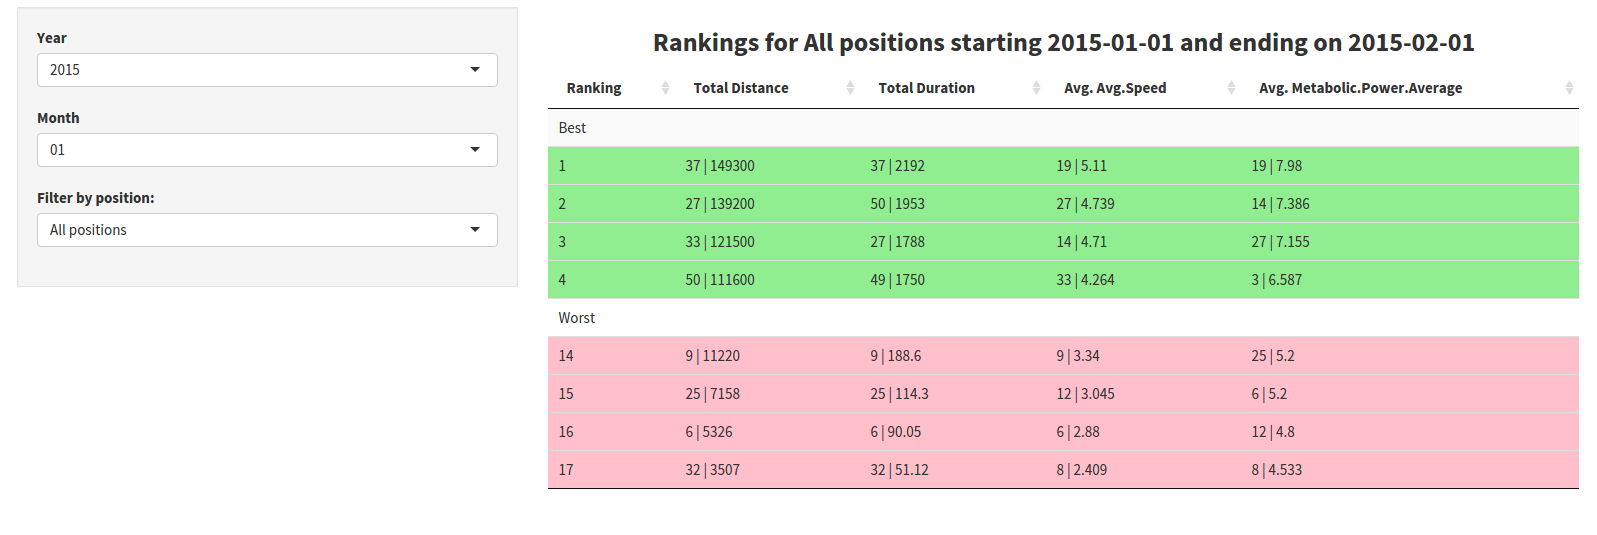
\includegraphics[height=4.5cm, width=10cm]{Images/RankingsTab.png}
	\caption{Rankings tab}
\end{wrapfigure}
The rankings tab was designed to display information about some key variables in the data in a compact and succinct manner. The figure was generated using the DT package in R. The user is given the choice to subset the time period to a month and the players who achieved the best and worst values in each key variable are highlighted. The name of the player is displayed beside the value that the player achieved for the variable over the time period. Again, care must be taken when using accumulative variables as the means of theses variables cannot accurately be compared.


\subsubsection{Report Downloader}
\begin{wrapfigure}{r}{9cm}
	\vspace{-2em}
	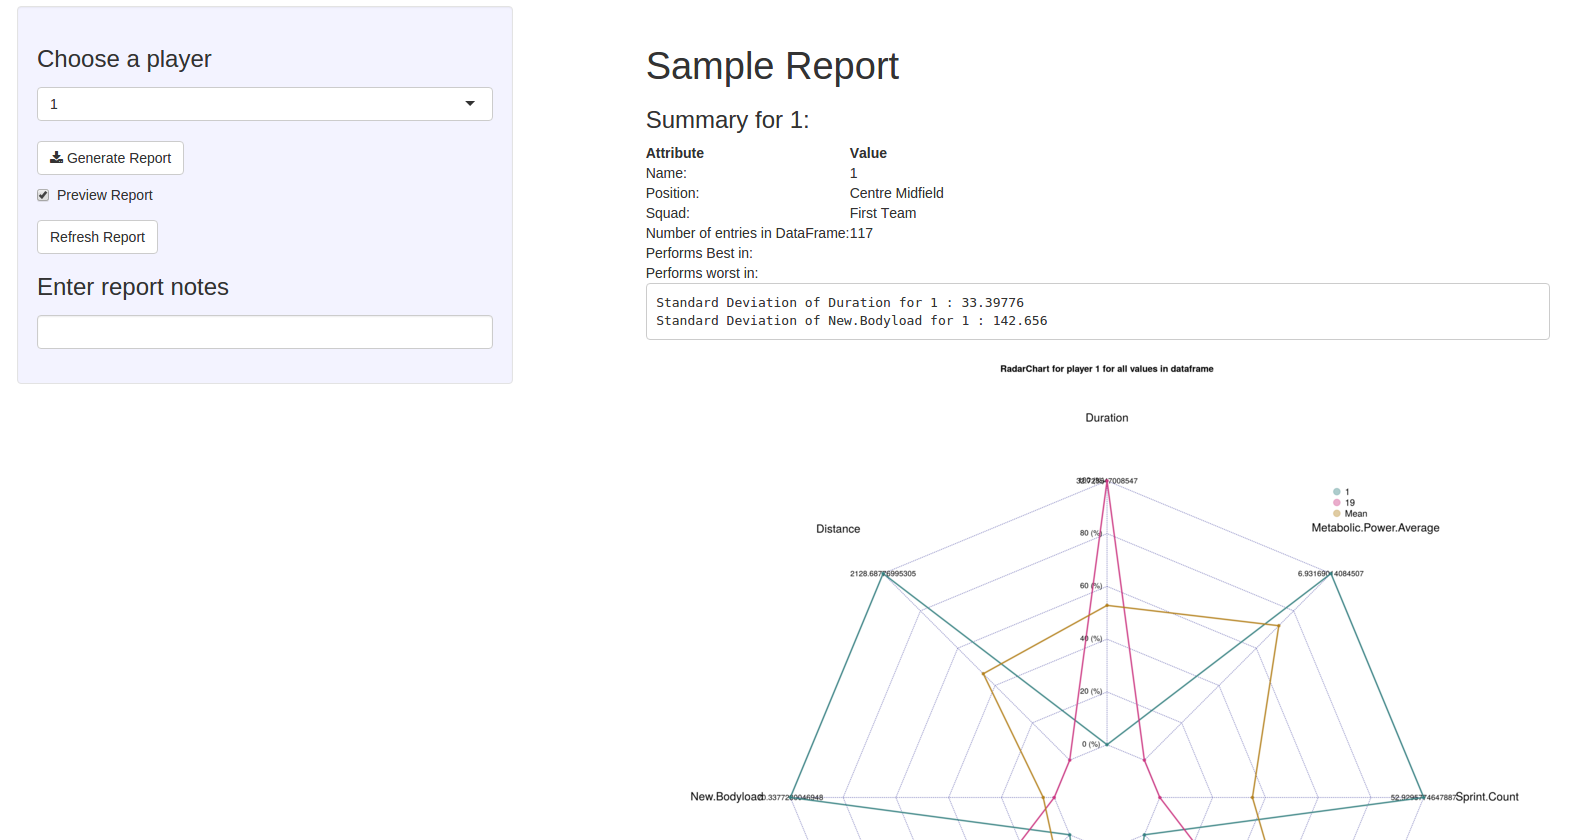
\includegraphics[height=5cm, width=10cm]{Images/DownloadReportTab.png}
	\caption{Report Download tab}
\end{wrapfigure}
The report Downloader tab facilitates the user entering some notes about a player and then downloading a customized report for that player. There is an option to view a rough preview of the report before downloading it, as shown in Figure 3.9. The report itself was generated using RMarkdown and introduces significant overhead to the App. A caching system for the reports or a separate report generating mechanism that runs in parallel to the application would be desirable for this tab, however to achieve this would take a considerable amount of code. There are also security issues related to downloading the report and the mechanism for storing the reports is currently flawed, meaning this is the only part of the application that would not run if deployed to a server.

\section{Dependencies}
Shiny's key strength is it's ability to display reactive output. This is facilitated using a series of outputs generated by the server function, which will automatically update when any of the inputs that the output relies on changes. This is referred to as dependency in a Shiny application. Dependencies are automatically created by the framework in order to track when an input variable changes so that the corresponding output remains up to date. The only requirement is that each input and output has a unique identifier in the App name space. Dependencies reflect the fundamental relationship between outputs and inputs. For example, in my application the player summary tables changed whenever the selected player changed, hence a dependency was set up on selected player. However, the programmer must be careful to only re-run code when necessary, otherwise a large overhead would be introduced making the program sluggish and frustrating to use. Shiny handles this by providing reactive functions, which come in three main flavours: reactive, render and observe, all of which were used in the application. 
\subsubsection{Reactive Expressions}
\begin{wrapfigure}{r}{4cm}
	\vspace{-2.5em}
	\caption{Example reactive expression \cite{shinyCheatSheet}\label{wrap-fig:1}}
	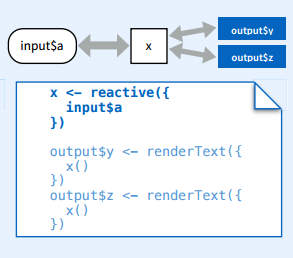
\includegraphics[height=3cm, width=4.5cm]{Images/ReactiveExpressionExample.png}
\end{wrapfigure}

The purpose of reactive expressions is to create objects that will be used in multiple outputs. Reactive expressions cache their evaluations the first time you run them. In subsequent calls, the reactive expression checks if the saved value needs to be updated (i.e., whether the inputs it depends on have changed). If the value does need to be updated, the reactive object will recalculate it and then cache the new result. If the value is already updated, the reactive expression will return the cached value without running the computations involved in the function \cite{shinyCheatSheet}. In my application, the Preprocess reactive expression took in data provided by the user and cleaned it so that it was in a suitable format for use throughout the rest of the server. Since this calculation took a few seconds to run in the application, using the cached value greatly boosted the App's responsiveness.
\begin{lstlisting}[language=R, basicstyle=\small]
Preprocess=reactive({
  #do all preprocessing, validation and error checking here and then
  #return processed data frame
  .....
  .....
  ProcessedData
})

\end{lstlisting}

\subsubsection{Observe Expressions}
\begin{wrapfigure}{r}{4cm}
	\vspace{-2.5em}
	\caption{Example observe expression \cite{shinyCheatSheet}}\label{wrap-fig:2}
	\includegraphics[height=3cm, width=4.5cm]{Images/ObserveExample.png}
\end{wrapfigure} 

Observe expressions create code that executes when an input changes, but do not directly create output objects. Observers are most often used for their side effects \cite{shinyCheatSheet}. For example, in my application I wanted the months drop down to only contain months that athletes trained in for the selected year. An observe expression was used to create a dependency on the barplotyear input. When the barplotyear input changed, the observer ran and updated the barplotMonth input, without returning anything.
\begin{lstlisting}[language=R, basicstyle=\small]
upDateBarplotMonths=observe({
  #Create dependency on barplotyear - when this changes, dates need to
  #update
  input$barplotYear
  validate(need(exists('ProcessedData'),""))
  updateSelectInput(session, "barplotMonth", 
  choices = sort(unique(format(as.Date(ProcessedData[format(as.Date(
  ProcessedData$Date,format="%Y/%m/%d"),'%Y')==input$barplotYear,'Date'],
   format="%Y/%m/%d"),"%m")))
  )
})
\end{lstlisting}
\newpage
\subsubsection{Render Expressions}
\begin{wrapfigure}{r}{4cm}
	\vspace{-2em}
	\caption{Example observe expression \cite{shinyCheatSheet}}\label{wrap-fig:2}
	\includegraphics[height=3cm, width=4.5cm]{Images/RenderExpression.png}
\end{wrapfigure} 

Render functions are used in shiny Apps to pass plots, charts, text and other output created in the server to the UI to be displayed. An output will automatically update whenever an input in its render function changes. Render expressions typically hold the code that the server needs to rebuild a UI component after a widget changes \cite{shinyCheatSheet}. Shiny uses the convention of naming render expressions as render[Output Type], where the output types range from tables to plots. Render expressions must return a specific type of object to be displayed or else errors are incurred. In my application, the render expressions tended to be lengthy since most of the plots are quite detailed, however a simple example exists in the form of the player summary table.
\begin{lstlisting}[language=R, basicstyle=\small]
output$PlayerSummaryPlot=renderTable({
  input$getname
  playerSummary(input$getname)
})
\end{lstlisting}

\subsubsection{Dependency Graph}
\begin{wrapfigure}{r}{5cm}
	\vspace{-2em}
	\caption{Render \& Observe Nodes (Endpoint)\cite{shinyCheatSheet}}
	\includegraphics[height=0.8cm, width=1.5cm]{Images/ReactOutput.png}
	\caption{Reactive Nodes (Intermediary)\cite{shinyCheatSheet}}
	\includegraphics[height=0.8cm, width=1.5cm]{Images/MidPoint.png}
	\caption{Input Nodes (Start Point)\cite{shinyCheatSheet}}
	\includegraphics[height=0.8cm, width=1.5cm]{Images/InputNode.png}
\end{wrapfigure}  
Shiny has many debugging tools and tricks that can help the application designer to ensure that their App is running as expected. One such tool is the reactive log visualization. This is essentially a dependency chart that shows how the outputs in an application depend on the inputs. There are three types of nodes in this chart displayed in figures 3.3-3.5. Figure 3.16 displays a dependency graph created before the App was completed. Notice that some nodes have many connections which denotes indicates their complexity in the application. Nodes exist that have no connections which shows that they are redundant in the application (which can be useful for debugging).
\begin{figure}[h]
	\includegraphics[width=18cm, height=10cm]{Images/ReactLog.png}
	\caption{Reactive Log Graph}
\end{figure}

\section{Program Work-flow}
Shiny applications execute according to the following sequence: 
\begin{enumerate}
	\item The UI file runs everything above the UI function once.
	\item The UI file runs the code inside the UI function once.
	\item The Server file runs the code above the Server function once.
	\item The Server file runs any code outside render, reactive or observe functions once.
	\item The Server file runs code inside reactive expressions multiple times according to the dependency list that Shiny has built up. Whenever an input in a reactive expression changes, the expression will re-run.
\end{enumerate}
The program was designed to comply with this work-flow. Auxiliary functions and other expressions that only need to be run once were defined outside of the server function in order to improve the responsiveness of the App. Reactive expressions contained the minimum amount of code that was required to update the application when a dependency changed in value.

\section{Testing}
As the App grew in complexity, it grew frustrating to alter some section of code and then manually run the App and check each tab to ensure that the App still operated as intended. I wrote a short set of unit tests in the python language using the selenium package in order to automate this process. This meant that every time I made a significant change to the App, I could run the tests while working on some other part of the application without having to manually ensure everything was present. I wrote the tests in python because the application needed to be running in order to use the selenium web driver to navigate it and because python is more suited to testing web applications than R. Code can be found for the tests on Github at \cite{AppTestFiles}.









	
	\newpage
	\chapter{Conclusion}
	The main challenge of this project for both the visualization and analysis was the high dimensionality of the data set. Building an application that can display information relating to each of the different aspects of the data was a task that required researching the domain in order to construct meaningful visualizations and then researching techniques that facilitate the implementation of these visualizations through a suitable platform. This was an iterative process that required refinement and revision at each step. The code found at \cite{ShinyServer} documents the order in which these revisions and improvements were carried out and is reflective of the chronological development of the App.
\hfill\break
\newline
Building an App that implemented the desired functionality but was also responsive, user friendly, extendable and scalable was a complex problem to tackle. From the outset of the development phase, I broke up this complex problem into many smaller, simpler sub-problems, while simultaneously designing an architecture for the App which could efficiently recombine the solutions to each of these sub-problems. This manifested itself as the modularization of the App into tabs which dealt with different aspects of the data separately. This meant that the App could be developed in incremental steps where editing, removing or adding a tab was independent of the existence of other tabs in the App. 
\hfill\break
\newline
The other main challenge in the development of the App was efficiently manipulating the data in order to display some aspect of the data. Complex filtering, subsetting, aggregating, splitting, mapping and recombining of the data was necessary to display most of the graphs in the App. These operations were dependent on user input, which added a further layer of complexity. The R functions apply, aggregate, paste, match, rbind, unique, ifelse, Reduce and append were used extensively to implement these operations. Packages such as TidyR could be explored in future to avoid the necessity of repeating these operations for multiple graphs by reshaping the data to a more convenient form as soon as it is read in by the App. Further work on this project could include deployment of the App to a server, improving the validation and error-checking/handling mechanisms, re-writing portions of the code to facilitate the usage of data sets from different sports and optimizing the responsiveness of the App.
\hfill\break
\newline
The statistical analysis of the New.Bodyload variable was also complicated by the high number of dimensions in the data. The ideal model was one that had few variables but also explained a high proportion of the variance relating to New.Bodyload, therefore a large part of the analysis focused on reducing the number of variables required in the statistical models. Multicollinearity of the predictors complicated this process, solutions to which were explored through orthogonalization techniques such as PCA and Partial Least Squares.
\hfill\break
\newline
The problem of identifying outliers in the data also consumed a large part of the time dedicated to the statistical analysis. As discussed in 2.4.1, I was not able to conclusively determine whether the suspected erroneous points were in fact erroneous, but I was able to suggest explanations for the generation of these points. Further analysis could have been performed on the process that generated these points, giving deeper meaning to the inferences developed. Another extension to this project would be to carry out a factor analysis, indicating the independent latent variables that account for most of the variability of other variables in the data, reducing the dimensionality of the data while retaining interpretability.
\hfill\break
\newline
Finally, it is also worth readdressing the fact that the data was gathered over time, meaning the observations were not independent from each other. Further analysis of New.Bodyload could involve exploring serial correlations over time, spectral analysis to examine cyclic behavior and fitting more complex models that takes the time component of the data into account in a more mature manner.





	
	\newpage		
	\begin{thebibliography}{1}
		\bibitem{StatsInSport}
		Prominence of Statistical Analyses in Sports
		\\\texttt{http://www.economist.com/node/2494781}
		\bibitem{GrowthOfStorageCap}
		Digital Data Storage Growth
		\\\texttt{http://www.eetimes.com/author.asp?section\_id=36\&doc\_id=1330462}
		\bibitem{tracking.pdf}
		GPSports FAQ
		\\\texttt{http://www.gpsports.com/support/FAQ\_GPS\_Tracking.pdf}
		\bibitem{shinyCheatSheet}
		Shiny Cheat Sheet
		\\\texttt{https://www.rstudio.com/wp-content/uploads/2015/02/shiny-cheatsheet.pdf}
		\bibitem{HadleyExploratoryAnalysis}
		R for Data Science
		\\\texttt{http://r4ds.had.co.nz/exploratory-data-analysis.html}
		\bibitem{GPSportsVariables}
		GPSports variables analysis
		\\\texttt{http://gpsports.com/gpsports-101/}
		\bibitem{NewBodyloadFAQ}
		GPSports New.Bodyload documentation
		\\\texttt{http://www.gpsports.com/support/UnderstandingBodyLoad.pdf}
		\bibitem{ISLR}
		An Introduction to Statistical Learning with Applications in R
		\\\texttt{http://www-bcf.usc.edu/~gareth/ISL/ISLR\%20Sixth\%20Printing.pdf}
		\bibitem{ESL}
		The Elements of Statistical Learning: Data Mining, Inference, and Prediction.
		\\\texttt{http://statweb.stanford.edu/~tibs/ElemStatLearn/}
		\bibitem{VIF}
		Detecting Multicollinearity Using Variance Inflation Factors
		\\\texttt{https://onlinecourses.science.psu.edu/stat501/node/347}
		\bibitem{Multicollinearity}
		Multicollinearity in Regression Models
		\\\texttt{\url{http://sites.stat.psu.edu/~ajw13/SpecialTopics/multicollinearity.pdf}}
		
		\bibitem{ModellingWithoutOutliers}
		Data Modeling file without suspected outliers
		\\\texttt{\url{https://github.com/DavidLSmyth/FinalYearProjectCode/blob/master/ModellingAndExplorationRFiles/RegressionModel.R}}
		
		\bibitem{ModellingWithOutliers}
		Data Modeling file with suspected outliers
		\\\texttt{\url{https://github.com/DavidLSmyth/FinalYearProjectCode/blob/master/ModellingAndExplorationRFiles/RegressionModelOutlier.R}}
		
		\bibitem{PreprocessingFile}
		Data Preprocessing \& Cleaning File
		\\\texttt{\url{https://github.com/DavidLSmyth/FinalYearProjectCode/blob/master/ModellingAndExplorationRFiles/PreprocessForPrediction.R}}
		
		\bibitem{ShinyServer}
		Shiny Server File
		\\\texttt{\url{https://github.com/DavidLSmyth/FinalYearProjectCode/blob/master/ShinyFiles/server.r}}
		
		\bibitem{ShinyUI}
		Shiny User Interface File
		\\\texttt{\url{https://github.com/DavidLSmyth/FinalYearProjectCode/blob/master/ShinyFiles/ui.r}}
		
		\bibitem{AppTestFiles}
		Testing Files for Shiny Application
		\\\texttt{\url{https://github.com/DavidLSmyth/FinalYearProjectCode/tree/master/testing}}
		
		
	\end{thebibliography}
\end{document}